\documentclass[a4paper]{article}

\usepackage[utf8]{inputenc}
\usepackage[T1]{fontenc}
\usepackage[french]{babel}
\usepackage{fullpage}
\usepackage{hyperref}
\usepackage{amsmath}
\usepackage{amssymb}
\usepackage{upgreek}
\usepackage{color}
\usepackage[]{algorithm2e}
\usepackage{stmaryrd}
\usepackage{graphicx}
\usepackage{float}
\usepackage{multirow}
\usepackage{subfig}
\usepackage{minted}
\usepackage[table]{xcolor}
\title{
    Assignment 3 : Multi-Armed Bandits\\
    \small INFO-F-409 - Learning Dynamics
}
\author{Florentin \bsc{Hennecker} (ULB 000382078)}
\date{}


\begin{document}
\maketitle

\section{N-Armed Bandit}
\subsection{Exercise 1}

Let us compare the performance of several algorithms trying to maximise the
reward they receive from an N-armed bandit which has 4 arms, each of which 
producing a reward sampled from a normal distribution of which the parameters
are shown in table \ref{banditparams}.

\begin{table}[H]
\centering
\begin{tabular}{c|c|c}
	\textbf{Arm} & $\mu$ & $\sigma$ \\
	\hline
	1 & 2.3 & 0.9\\
	2 & 2.1 & 0.6\\
	3 & 1.5 & 0.4\\
	4 & 1.3 & 2\\
\end{tabular}
\caption{Parameters of the 4-armed bandit}
\label{banditparams}
\end{table}

The algorithms to compare are $\epsilon$-greedy with parameters 0, 0.1 and 0.2,
Softmax with temperatures 1 and 0.1, and the random action selection policy.
Figure \ref{ex11perf} shows how each of these algorithms manage to maximise
their reward after playing for many iterations. 
\begin{figure}[H]
	\centering
	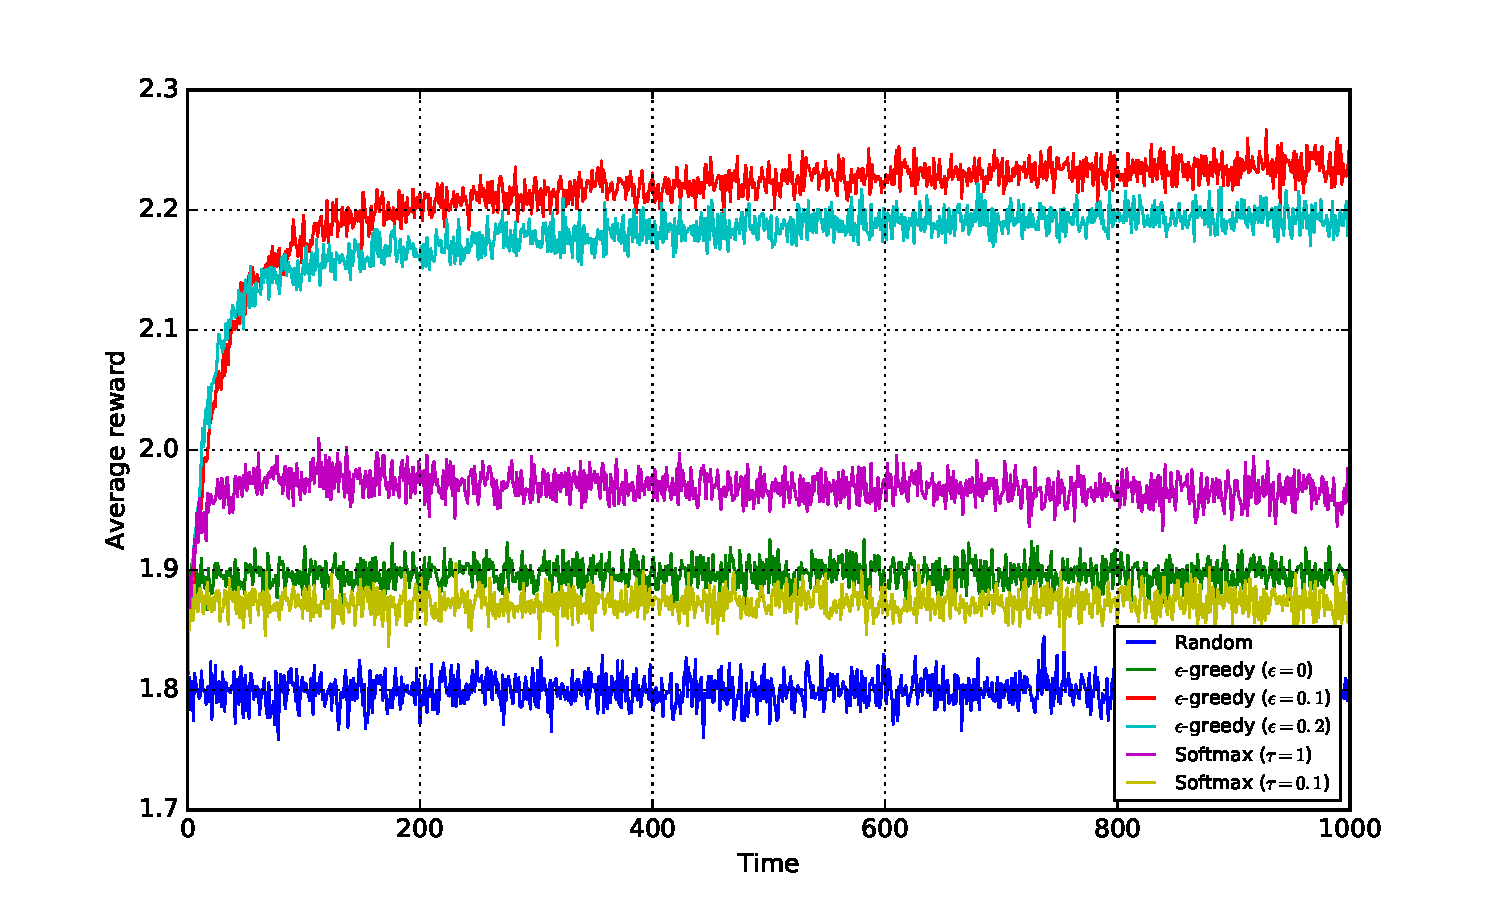
\includegraphics[width=0.7\textwidth]{./fig/ex1-1.pdf}
	\caption{Evolution of the average reward over 10000 runs during training}
	\label{ex11perf}
\end{figure}
As we can see, only two algorithms managed to converge to the best arm : 
$\epsilon$-greedy 0.1 and 0.2. Let us first explain the behaviour of 
$\epsilon$-greedy 0. It selects its first action at random, but for all the
following iterations, it will choose it again as its Q-value will be non-zero
and there is no room to explore. If all the arms had negative $Q^*_{ai}$, 
$\epsilon$-greedy would however pick the less negative one after it has explored
all of the actions.\\

Softmax outperforms the random selection policy but does not do very well. 
This is likely caused by the fact that there is a lot of noise in the rewards
and that the discrete distribution regulating the choice of action is fairly
homogeneous. This hypothesis can be confirmed by looking at figures 
\ref{ex11q} and \ref{ex11a}.

\begin{figure}[H]
	\centering
	\subfloat[][Arm 1]{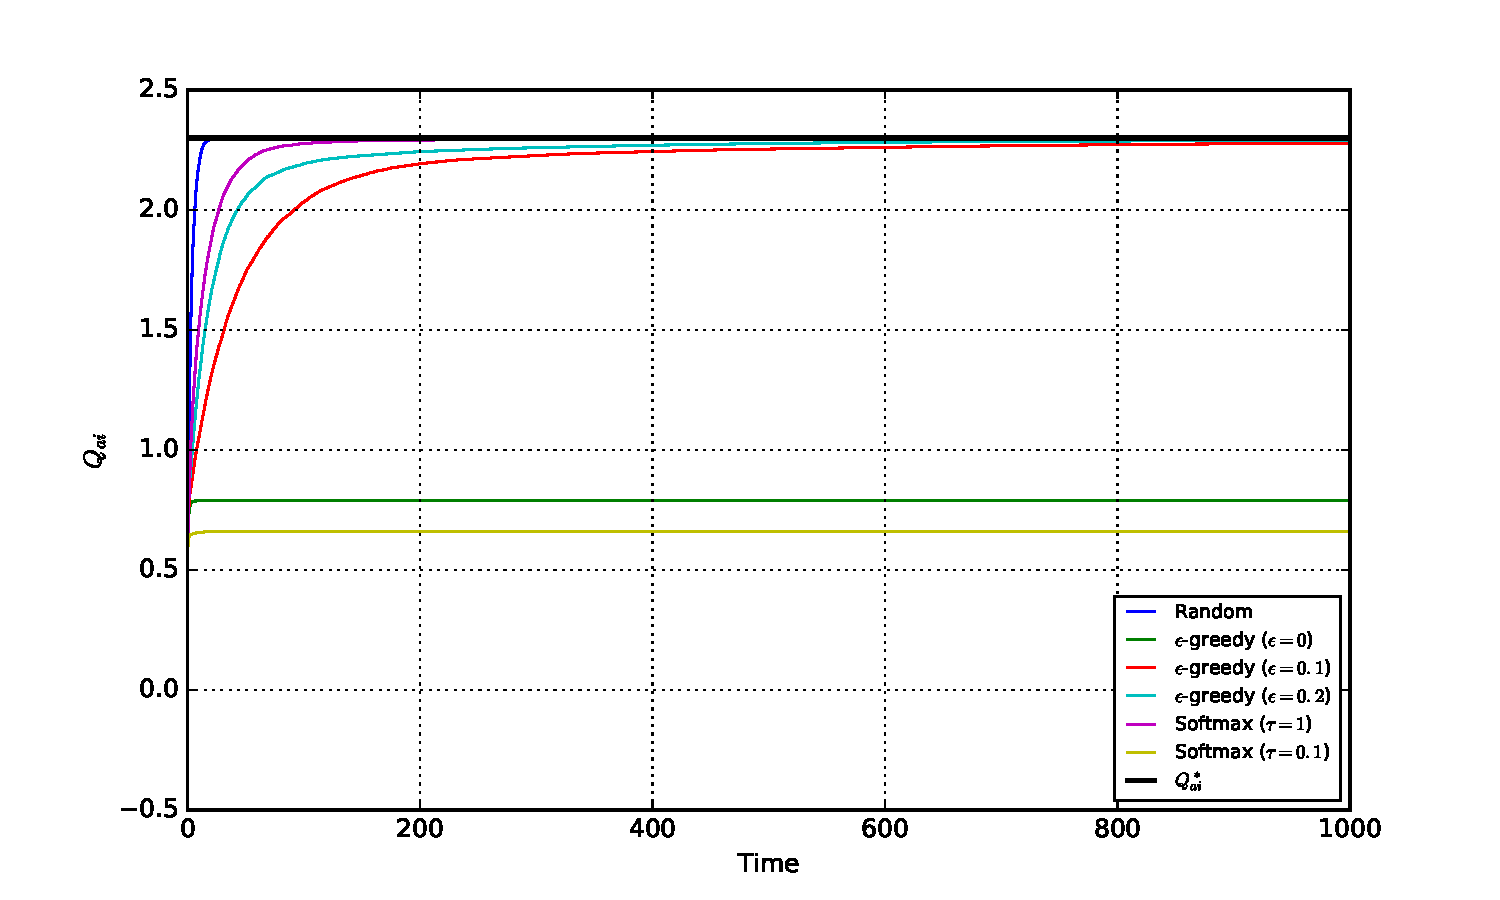
\includegraphics[width=.49\textwidth]{./fig/ex1-1-q0.pdf}}
	\subfloat[][Arm 2]{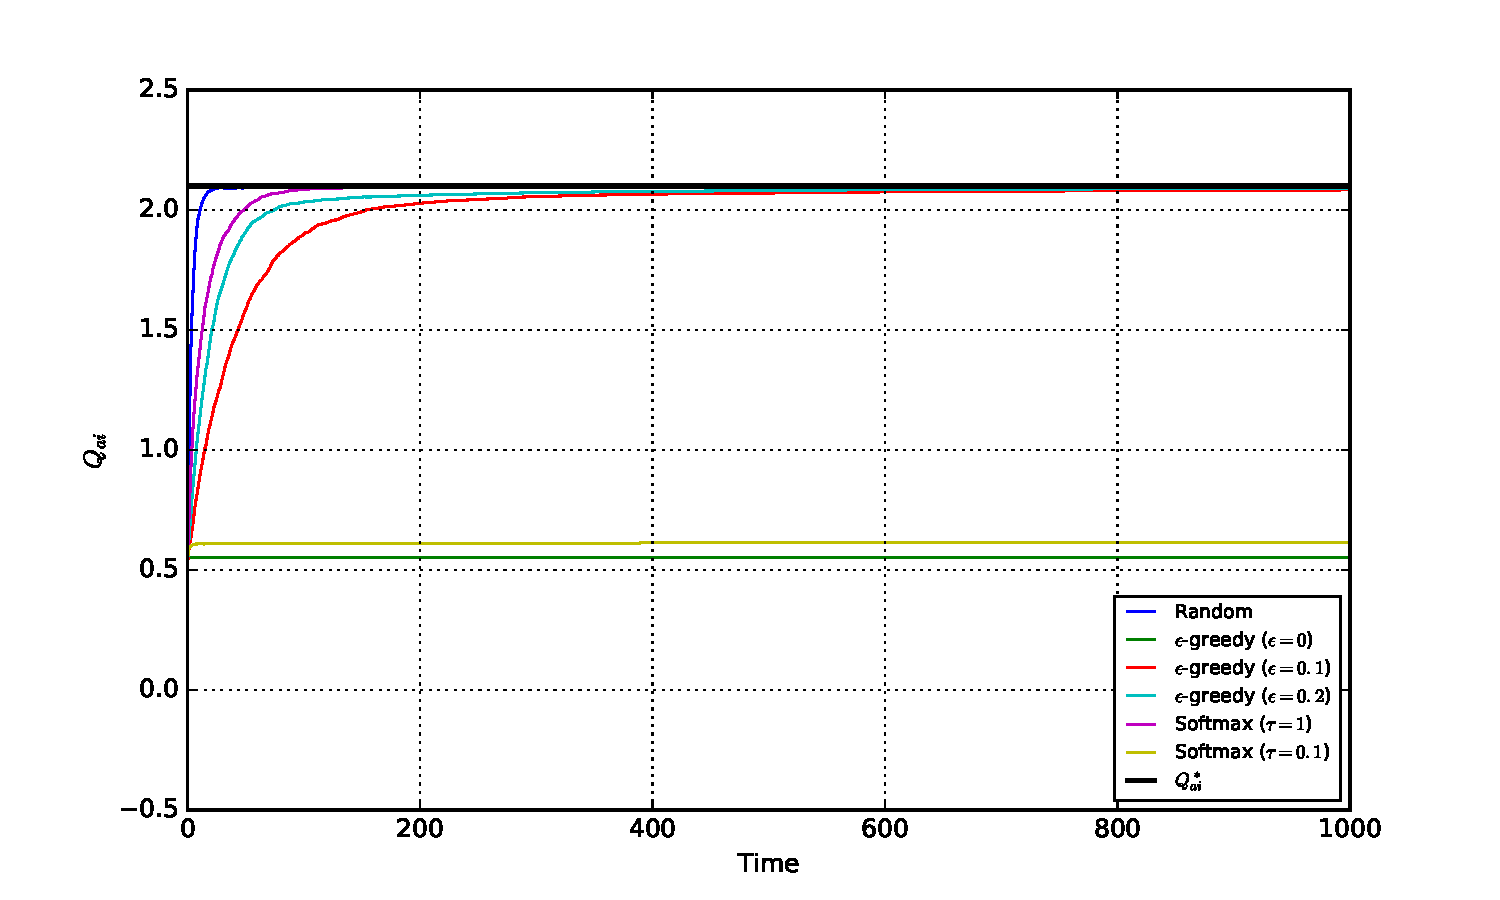
\includegraphics[width=.49\textwidth]{./fig/ex1-1-q1.pdf}}
	\\
	\subfloat[][Arm 3]{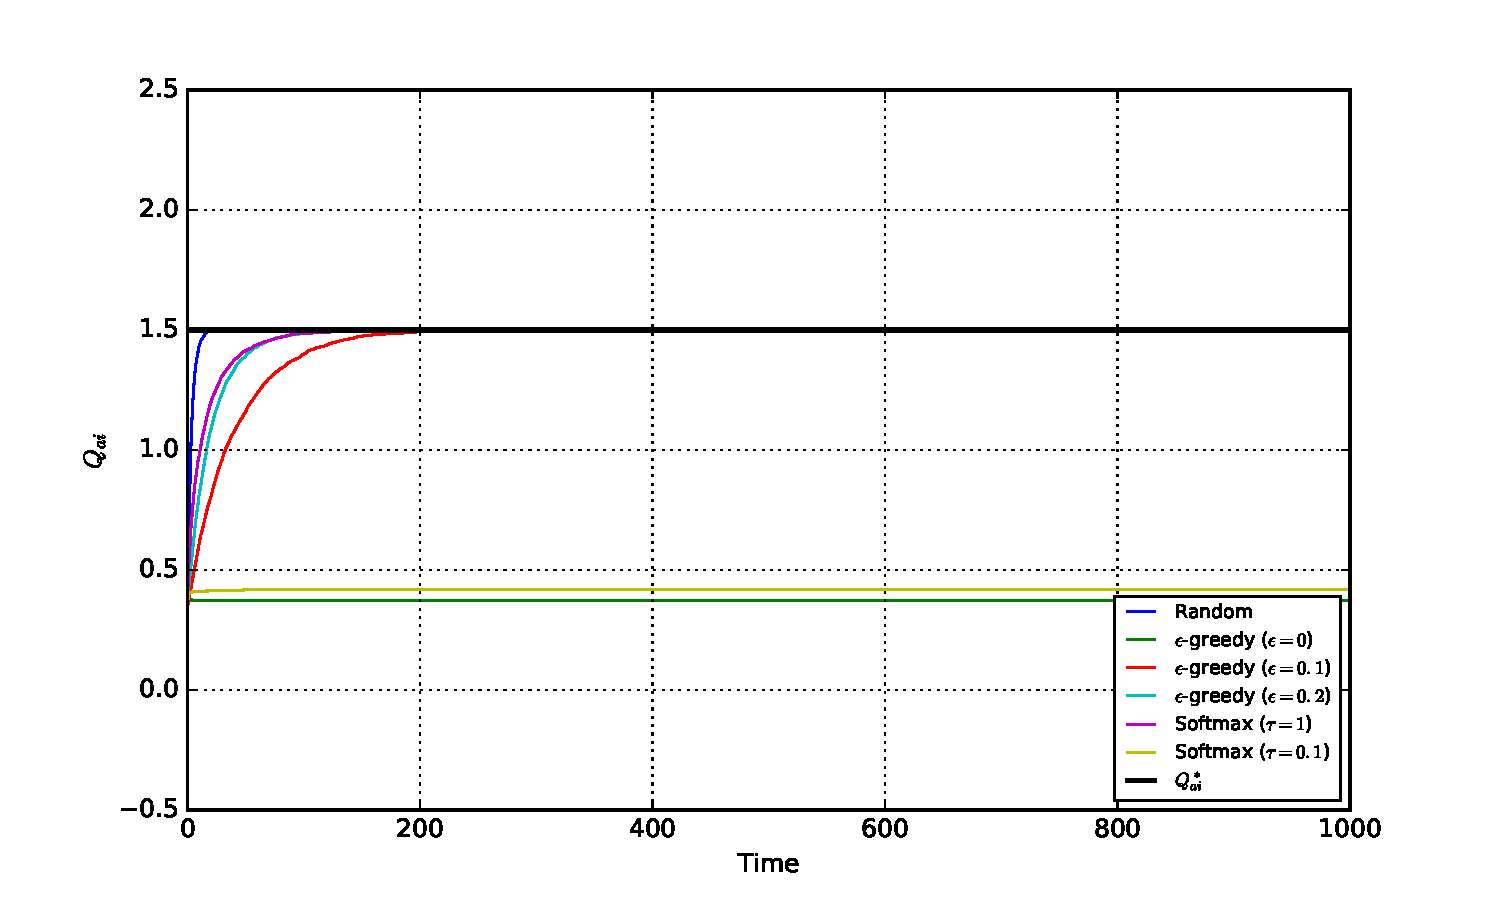
\includegraphics[width=.49\textwidth]{./fig/ex1-1-q2.pdf}}
	\subfloat[][Arm 4]{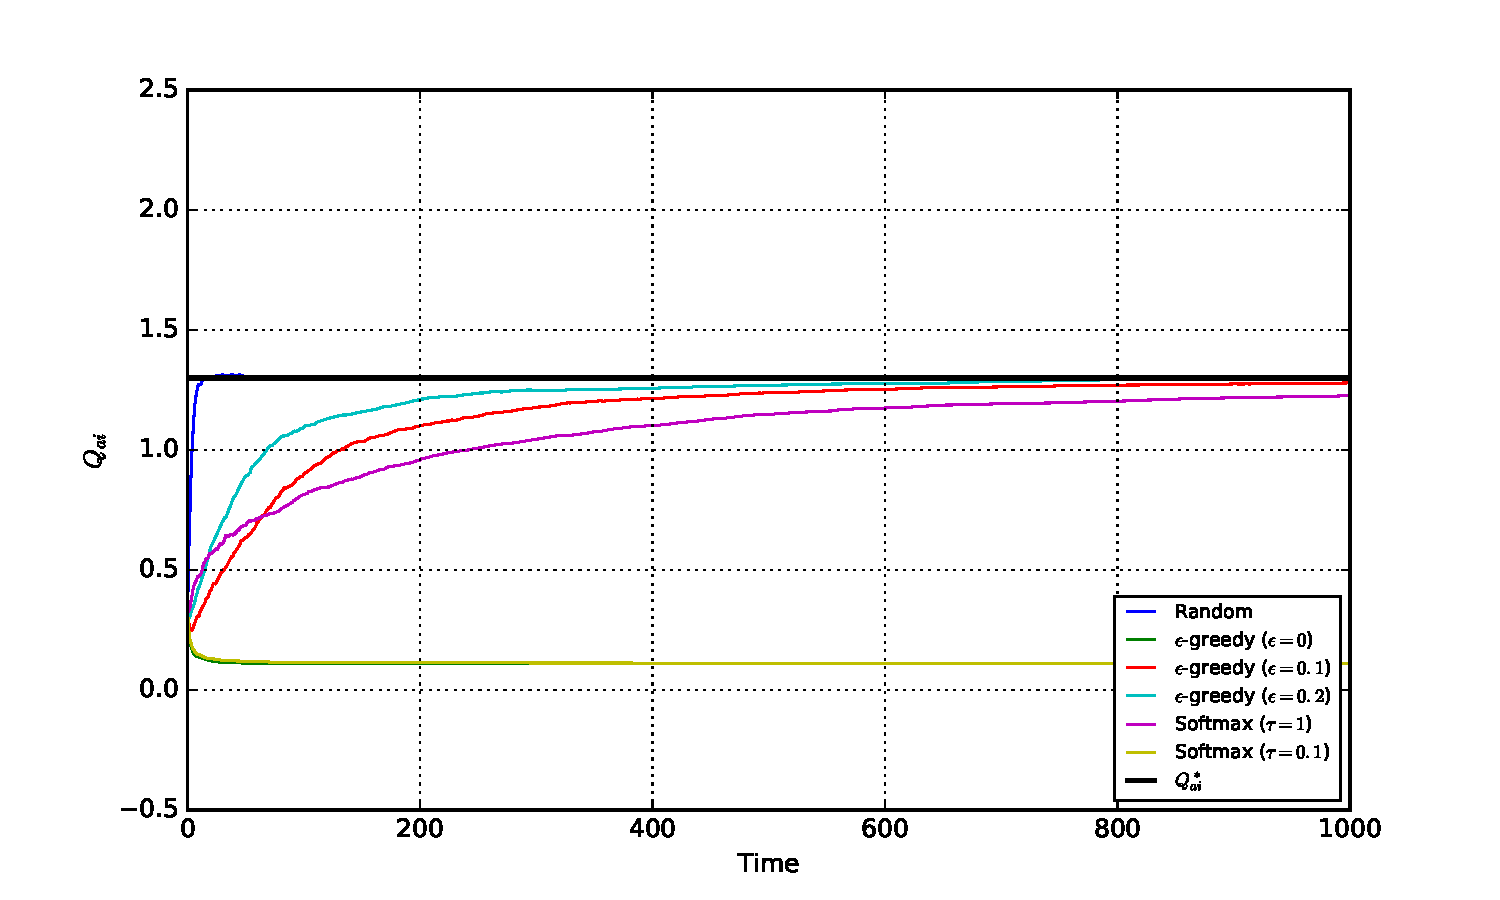
\includegraphics[width=.49\textwidth]{./fig/ex1-1-q3.pdf}}
	\caption{Evolution of $Q_{ai}$ for each arm}
	\label{ex11q}
\end{figure}

The first thing to note on figure \ref{ex11q} is that the random selection 
policy estimates $Q^*_{ai}*$ quite precisely very fast for each arm, which is
normal. One could say that random exploration is very good, but it only is at
the very start and for small problems with small action-state spaces.\\

Another interesting trend is that the best arm gets learnt much faster than the
worst one. This is due to the fact that the learning algorithms should pick it
more often, therefore allowing us to understand quicker its reward
distribution.\\

As for the speed at which each algorithm converges, it makes sense to see that
the higher $\epsilon$ is, the quicker it will converge because it follows a
more random behaviour. Softmax 1 has an interesting behaviour. It learns
very quickly about the quality of the good arms but much slower about the bad
ones.\\

Softmax 0.1 seems to have trouble learning this problem. In fact, it doesn't
have enough exploration power and will behave just like $\epsilon$-greedy 0.
Both will pick an action at the start and will stick with it until then end.
The graphs of figure \ref{ex11q} do not convey the idea that both algorithms
will actually learn the value of one arm very quickly, but leave the others at
0; this is due to the fact that each graph shows an average of many runs.\\

We have the same issue on figure \ref{ex11a} : it looks like all actions are
being taken roughly the same amount of time during a run, but both algorithms
actually only pick one (or almost one for Softmax 0.1) action for the whole run
and what we see is the fact that the action picked is picked at random at the 
start.

\begin{figure}[H]
	\centering
	\subfloat[][Random]{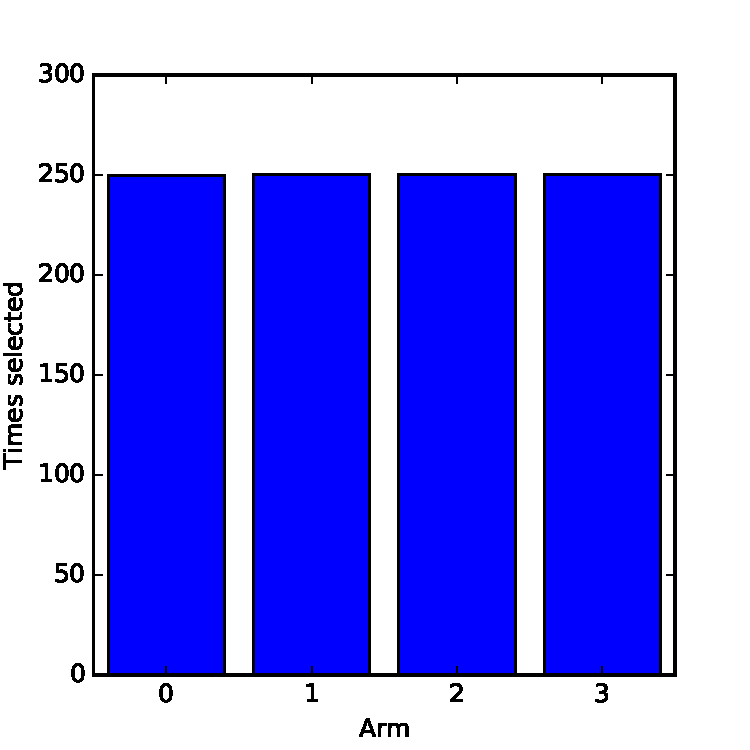
\includegraphics[width=.16\textwidth]{./fig/ex1-1-a0.pdf}}
	\subfloat[][$\epsilon$-greedy 0]{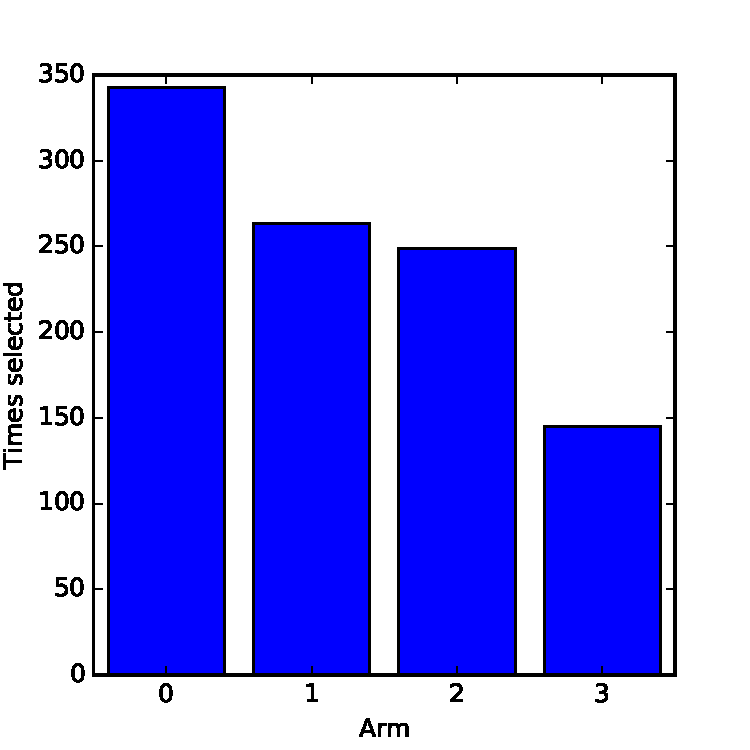
\includegraphics[width=.16\textwidth]{./fig/ex1-1-a1.pdf}}
	\subfloat[][$\epsilon$-greedy 0.1]{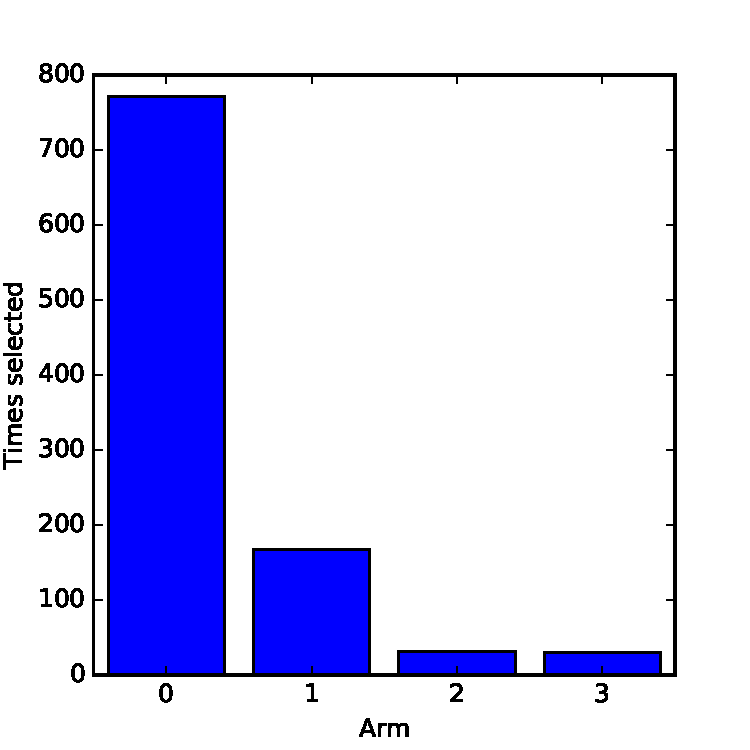
\includegraphics[width=.16\textwidth]{./fig/ex1-1-a2.pdf}}
	\subfloat[][$\epsilon$-greedy 0.2]{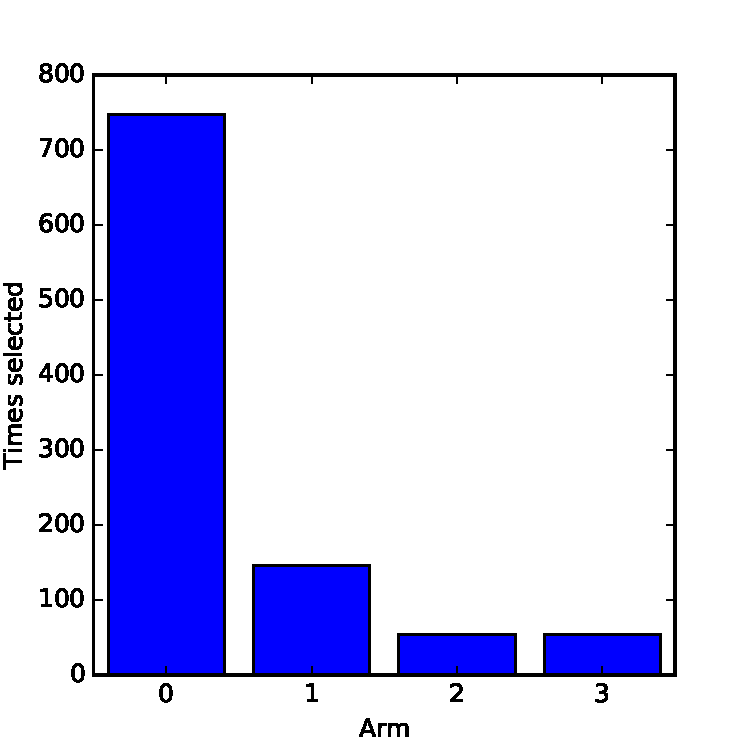
\includegraphics[width=.16\textwidth]{./fig/ex1-1-a3.pdf}}
	\subfloat[][Softmax 1]{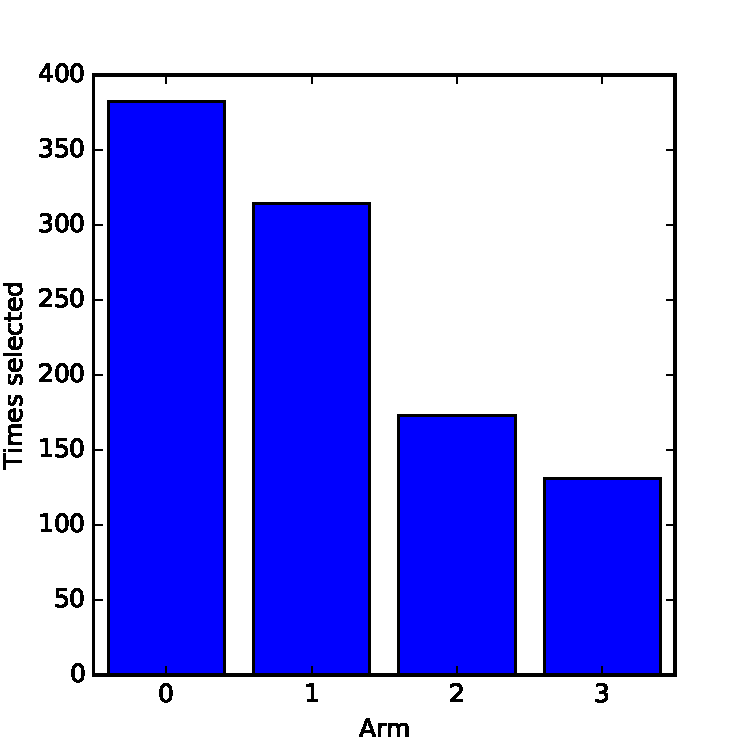
\includegraphics[width=.16\textwidth]{./fig/ex1-1-a4.pdf}}
	\subfloat[][Softmax 0.1]{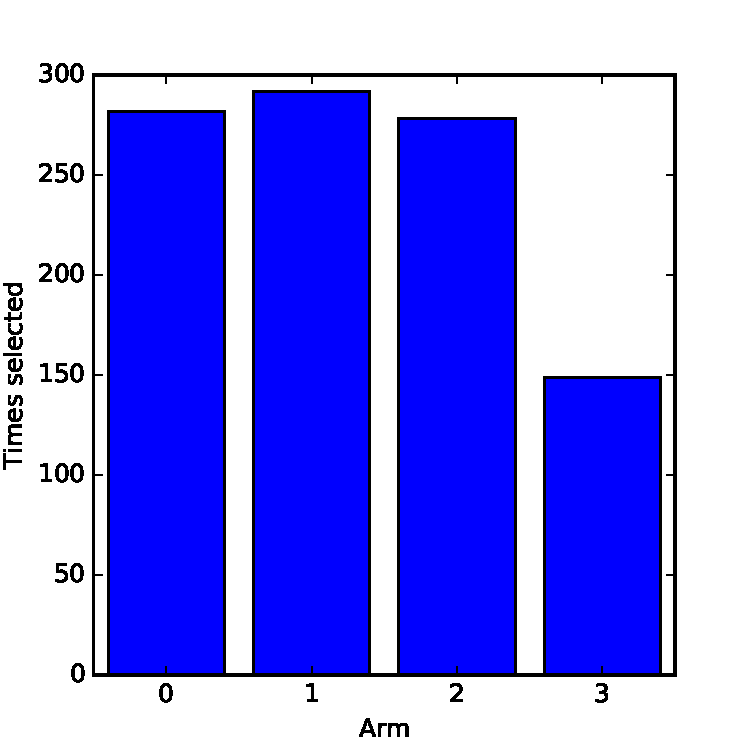
\includegraphics[width=.16\textwidth]{./fig/ex1-1-a5.pdf}}
	\caption{Actions taken by each algorithm}
	\label{ex11a}
\end{figure}

Concerning $\epsilon$-greedy 0.1 and 0.2, we clearly see that both algorithms
have learnt that the first arm is the best one. Also, with a higher $\epsilon$, 
the non-optimal actions get chosen a bit more. Softmax 1 seems to have learnt
that the best arm is the first one too but has a too high temperature to
always choose the best arm. 

\subsection{Exercise 2}
If we do the exact same exercise but double the standard deviation of the reward
for each arm, we see on figure \ref{ex12perf} that it is a harder problem to 
learn.
\begin{figure}[H]
	\centering
	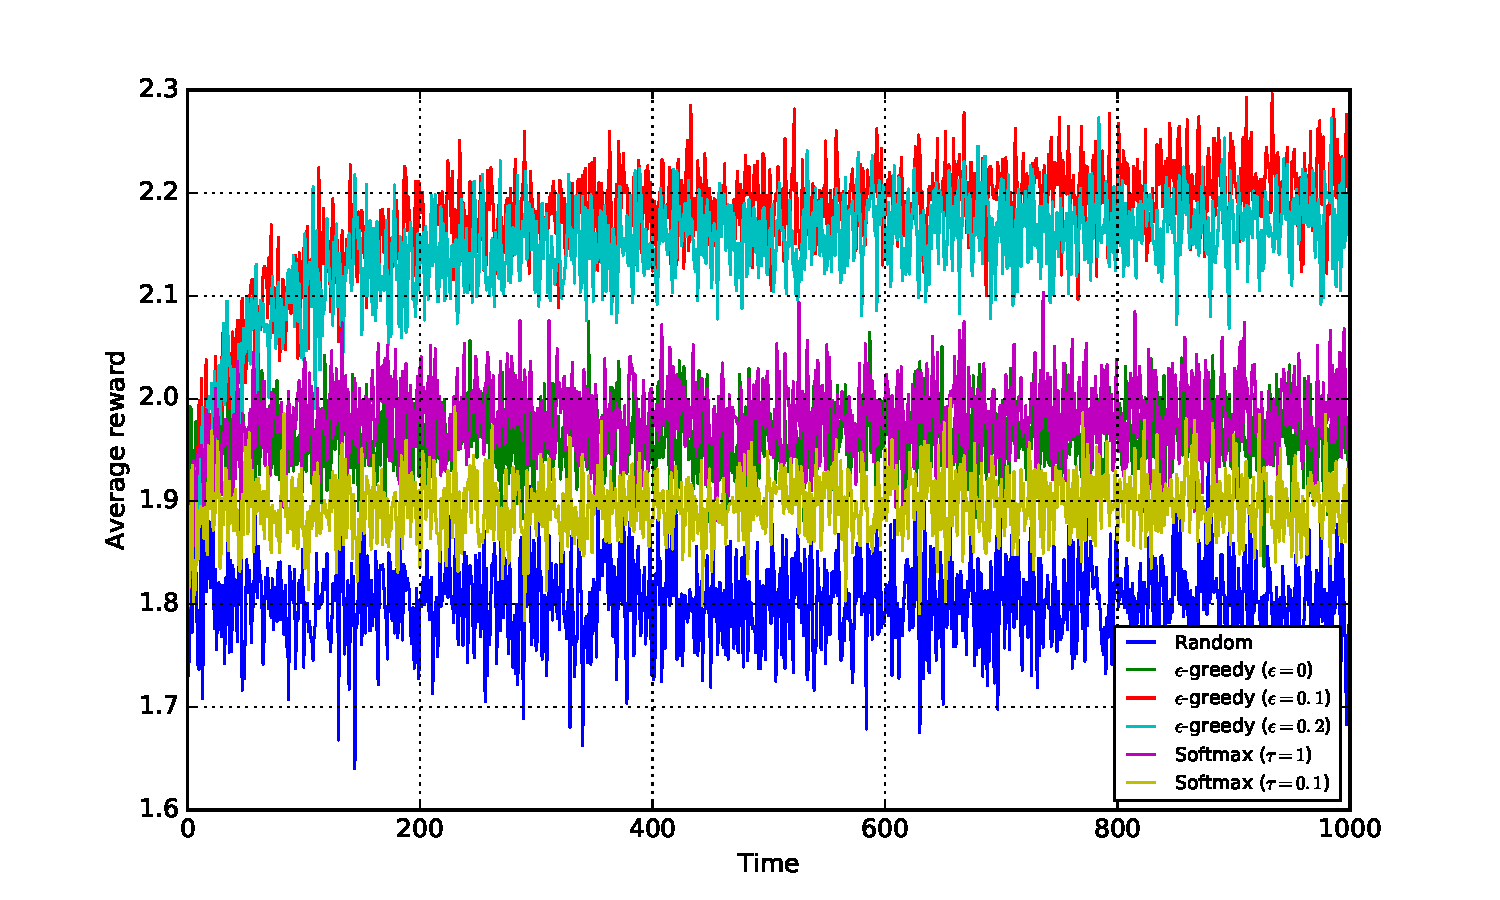
\includegraphics[width=0.7\textwidth]{./fig/ex1-2.pdf}
	\caption{Evolution of the average reward over 10000 runs during training}
	\label{ex12perf}
\end{figure}
When we compare this graph to the one shown in figure \ref{ex11perf}, we
notice that the variance of each learning curve is higher, but most importantly,
we see that the two algorithms that manage to train correctly learn slower. 
The average reward climbs above 2.2 before 200 iterations in the first case,
and it takes a lot more time in the second case. However, after 1000 iterations,
the difference is small; and it is for all the algorithms.\\

The fact that this problem is harder to learn is visible on figure \ref{ex12q}
too : all algorithms take more time to converge to the true values. The last
(and worst) arm is notably different. All algorithms (except the random one)
underestimate fairly wildly its value.\\

The graphs of figure \ref{ex12a}, although they are a bit more homogeneous for
$\epsilon$-greedy 0.1 and 0.2, are barely different than the ones of figure
\ref{ex11a}.

\begin{figure}[H]
	\centering
	\subfloat[][Arm 1]{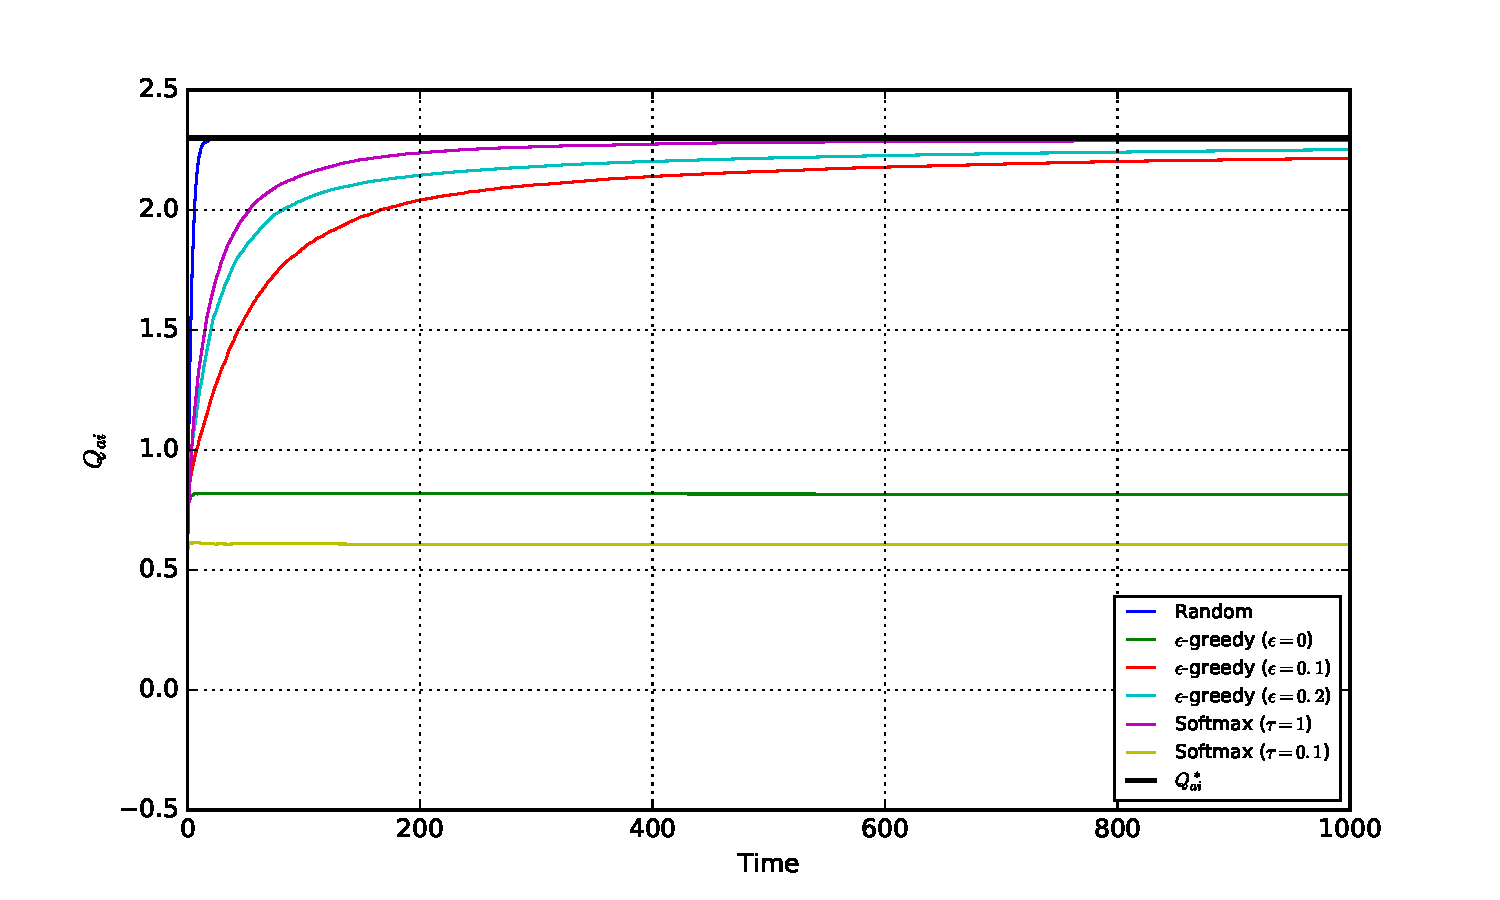
\includegraphics[width=.49\textwidth]{./fig/ex1-2-q0.pdf}}
	\subfloat[][Arm 2]{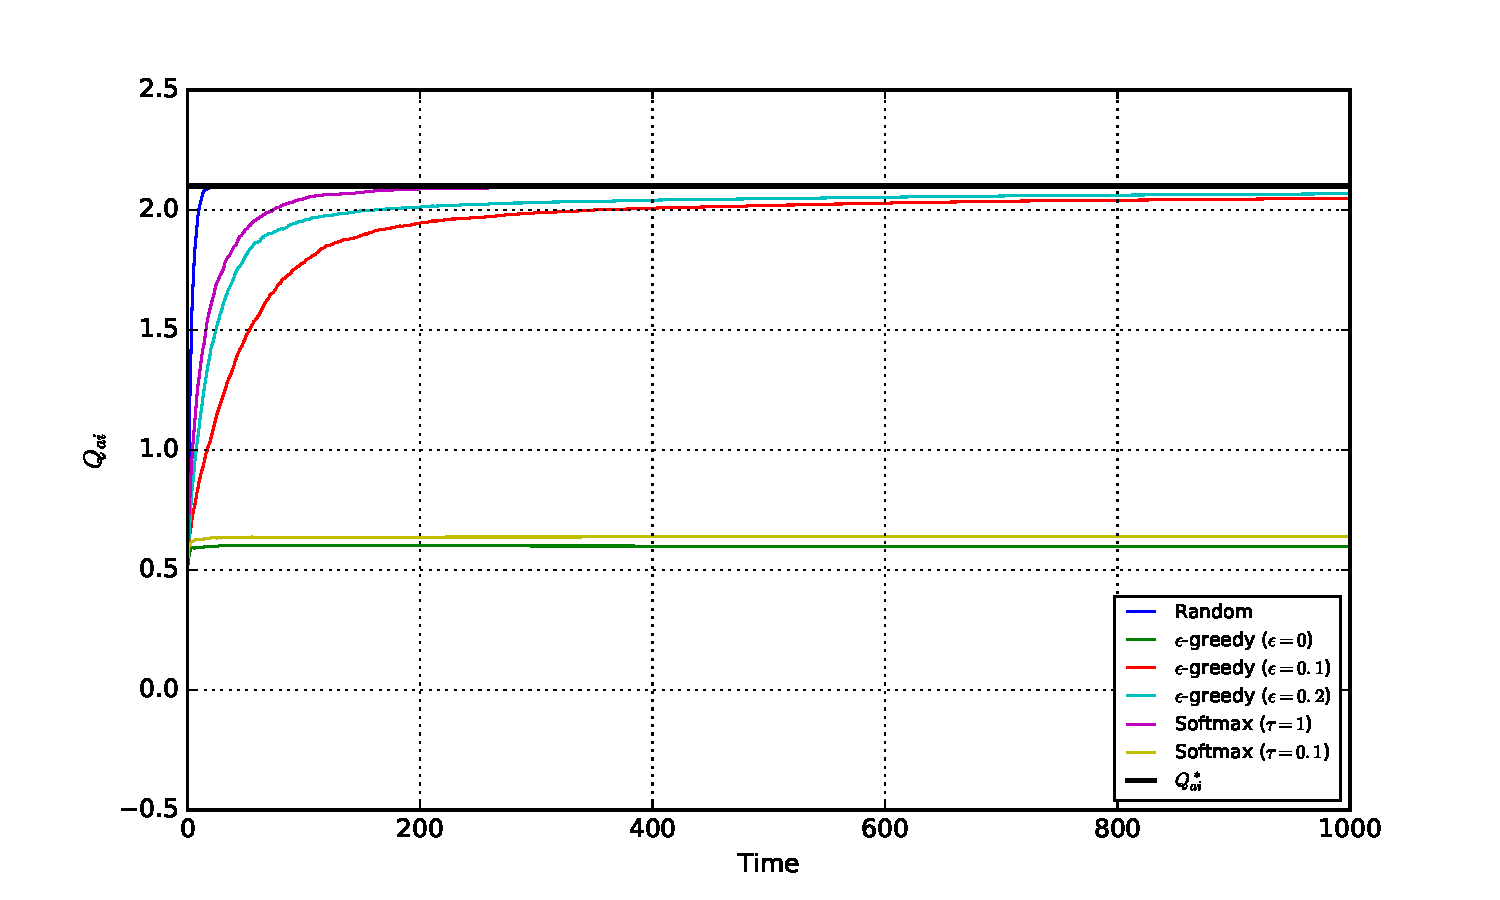
\includegraphics[width=.49\textwidth]{./fig/ex1-2-q1.pdf}}
	\\
	\subfloat[][Arm 3]{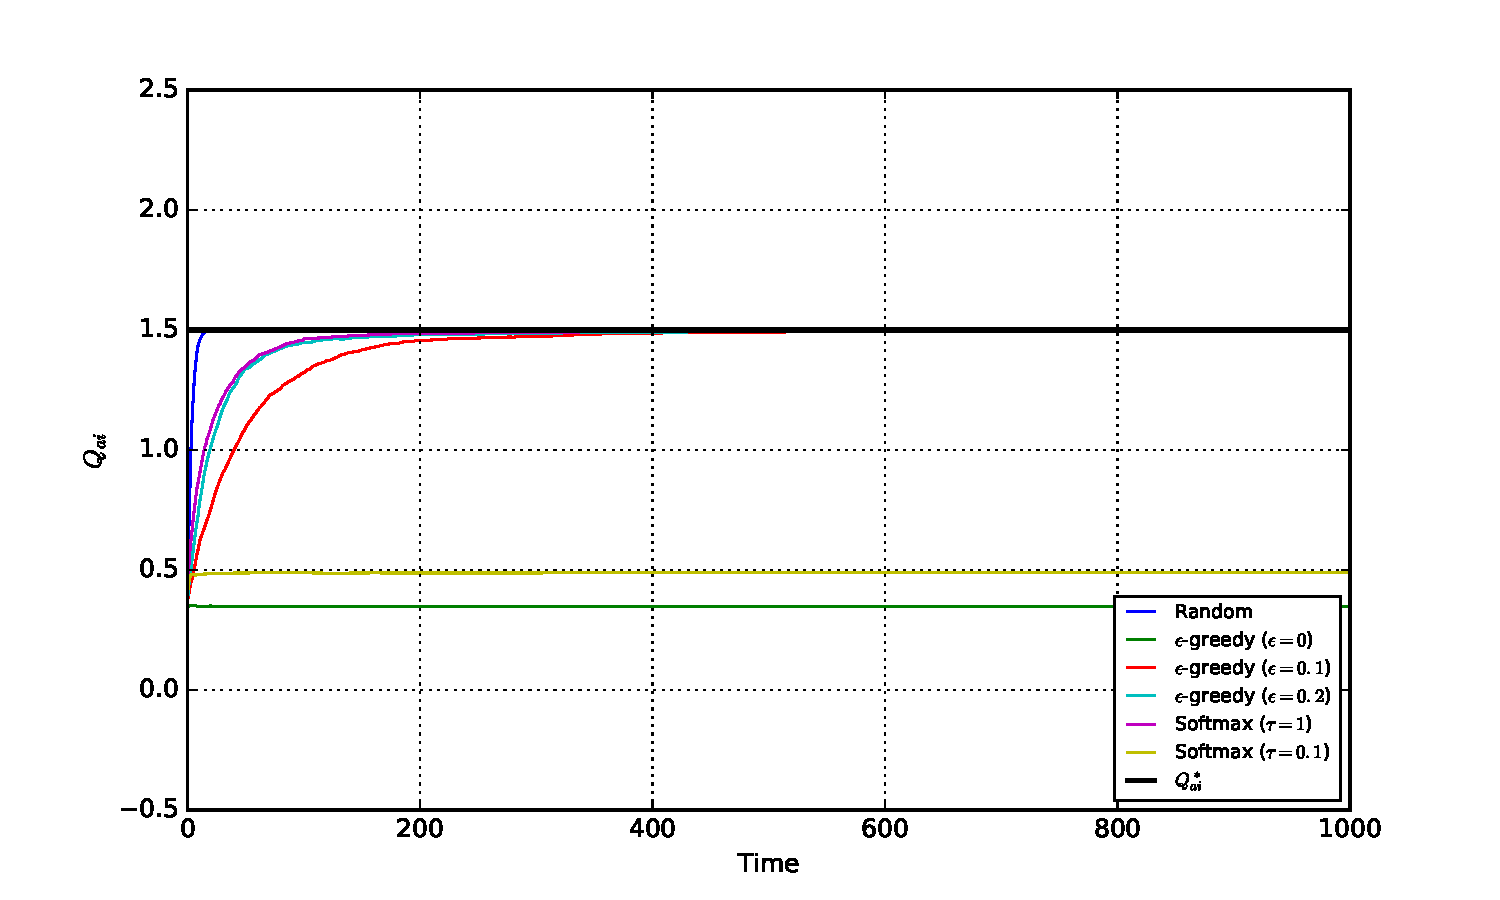
\includegraphics[width=.49\textwidth]{./fig/ex1-2-q2.pdf}}
	\subfloat[][Arm 4]{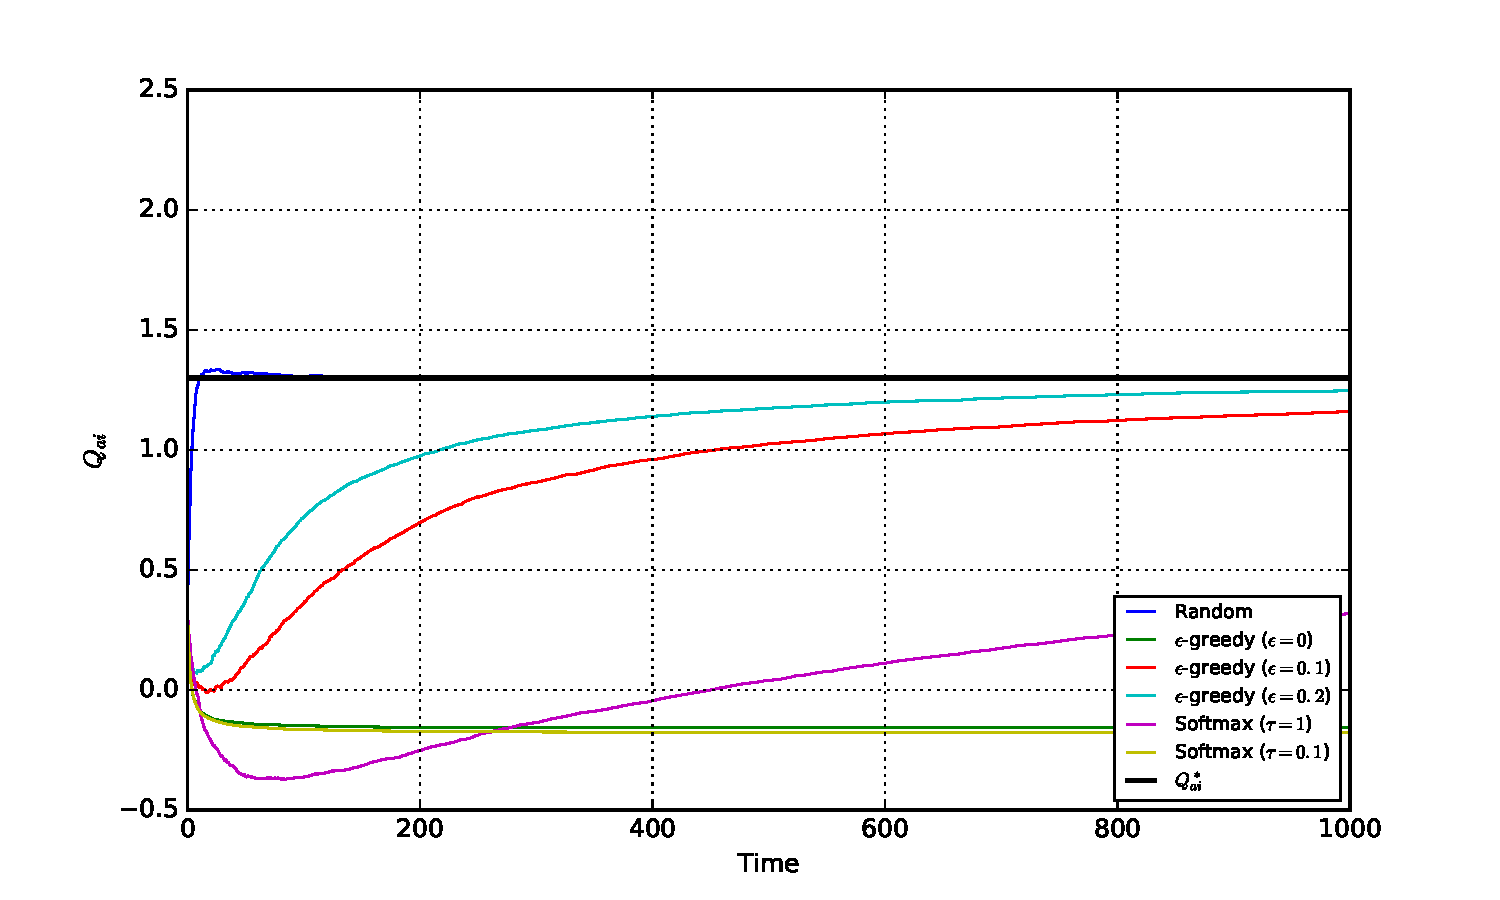
\includegraphics[width=.49\textwidth]{./fig/ex1-2-q3.pdf}}
	\caption{Evolution of $Q_{ai}$ for each arm}
	\label{ex12q}
\end{figure}
\begin{figure}[H]
	\centering
	\subfloat[][Random]{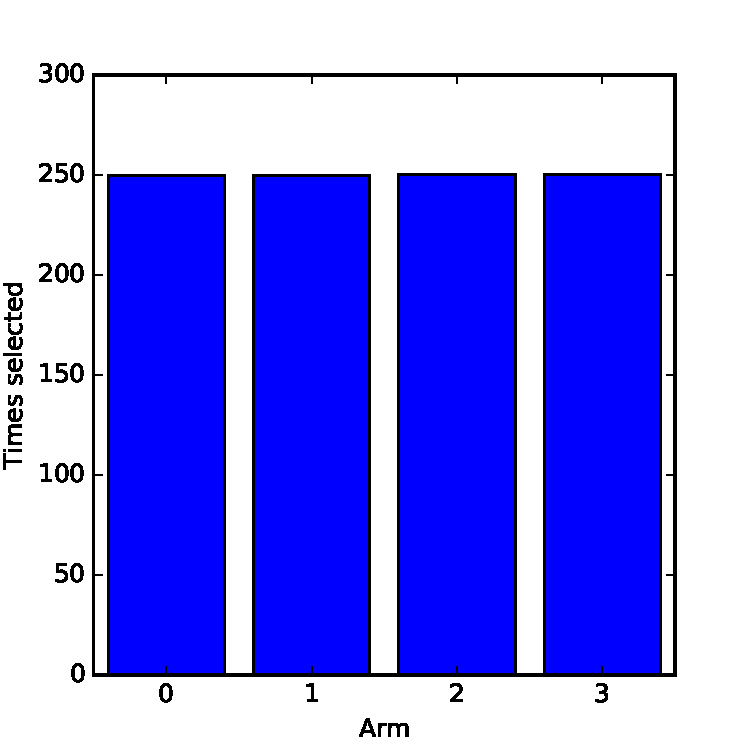
\includegraphics[width=.16\textwidth]{./fig/ex1-2-a0.pdf}}
	\subfloat[][$\epsilon$-greedy 0]{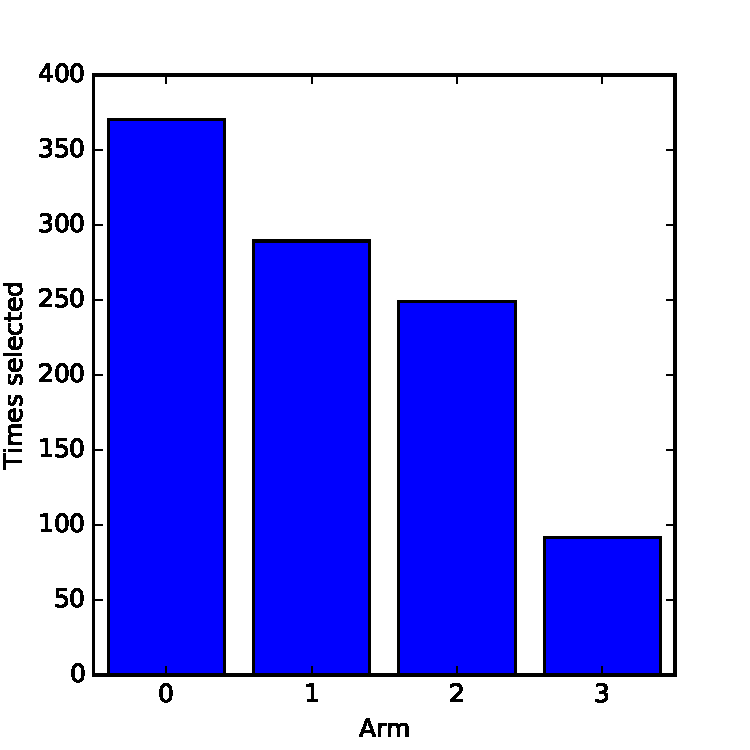
\includegraphics[width=.16\textwidth]{./fig/ex1-2-a1.pdf}}
	\subfloat[][$\epsilon$-greedy 0.1]{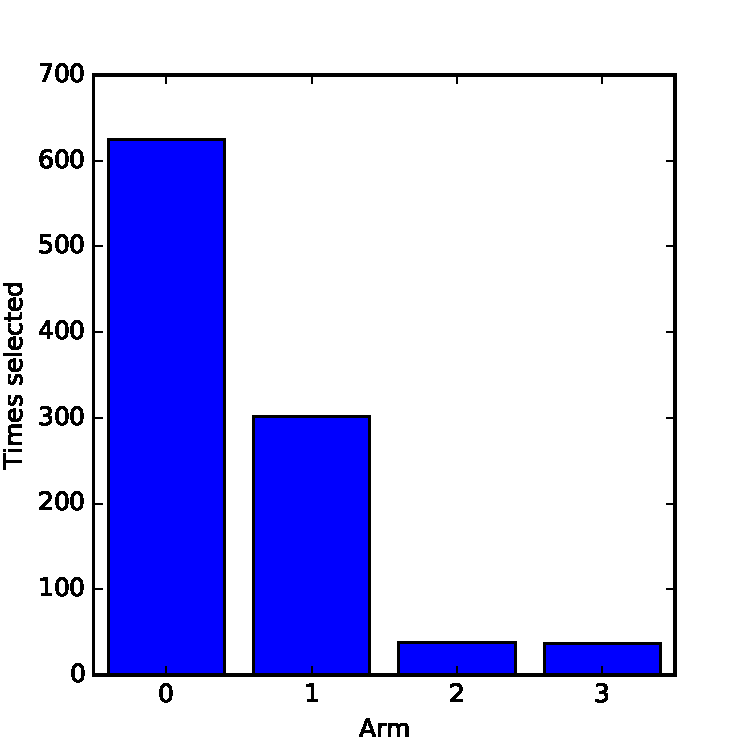
\includegraphics[width=.16\textwidth]{./fig/ex1-2-a2.pdf}}
	\subfloat[][$\epsilon$-greedy 0.2]{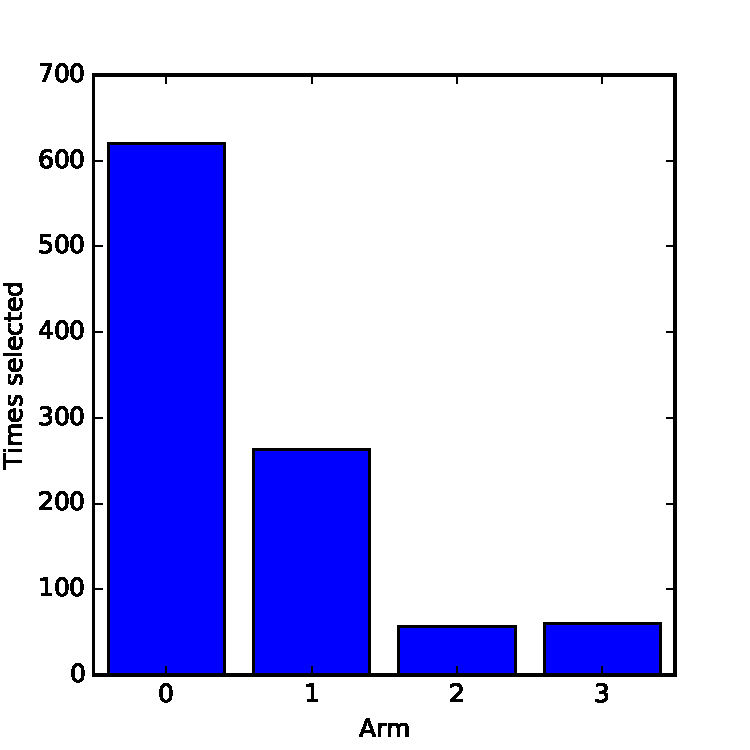
\includegraphics[width=.16\textwidth]{./fig/ex1-2-a3.pdf}}
	\subfloat[][Softmax 1]{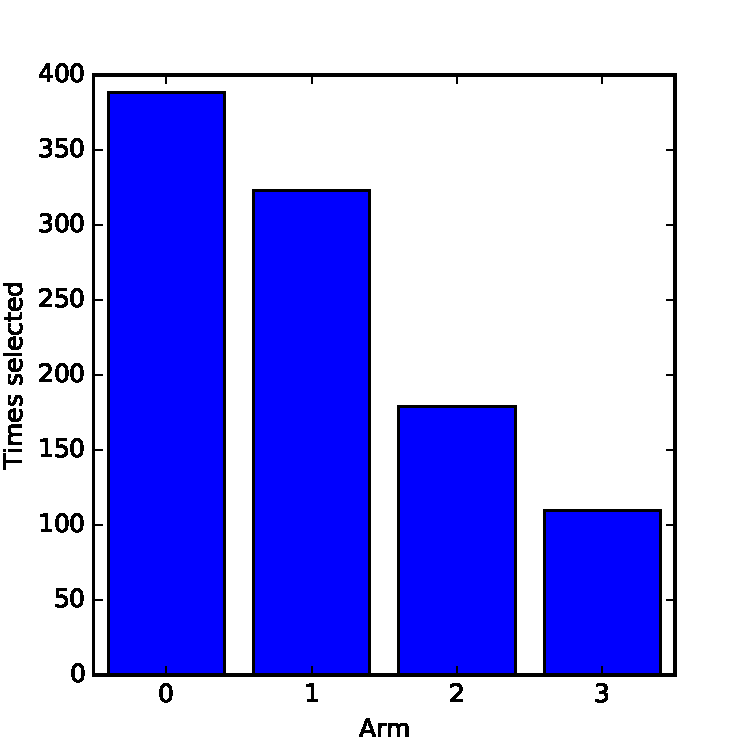
\includegraphics[width=.16\textwidth]{./fig/ex1-2-a4.pdf}}
	\subfloat[][Softmax 0.1]{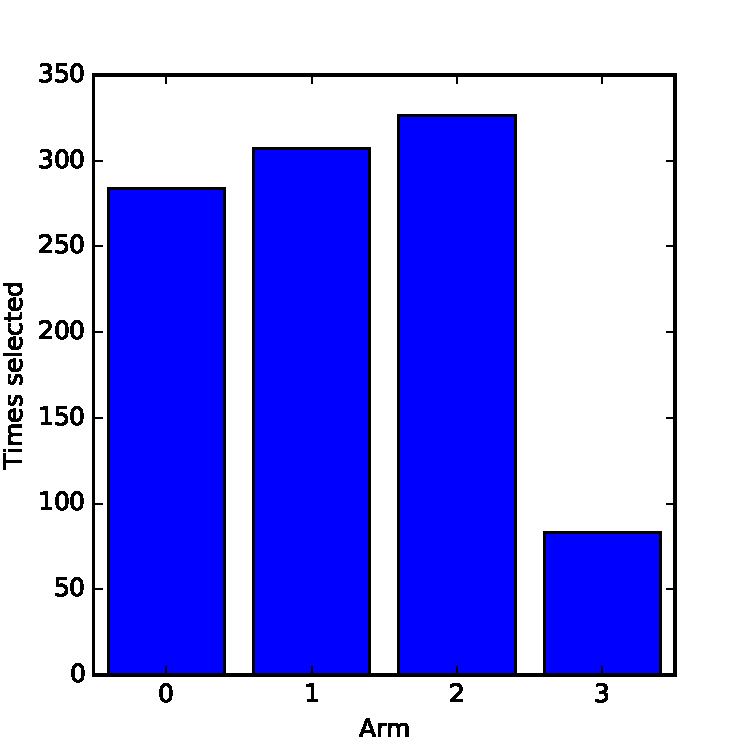
\includegraphics[width=.16\textwidth]{./fig/ex1-2-a5.pdf}}
	\caption{Actions taken by each algorithm}
	\label{ex12a}
\end{figure}

\subsection{Exercise 3}
Let us now compare $\epsilon$-greedy and Softmax with varying time parameters
on the problem posed in the first exercise. We will implement and compare:
\begin{itemize}
	\item $\epsilon$-greedy with $\epsilon = 1/\sqrt{t}$
	\item Softmax with $\tau = 4*\frac{1000-t}{1000}$
\end{itemize}

\paragraph{$\epsilon$-greedy} performs better than its fixed $\epsilon$ variants
on every aspect : it converges quicker, and reaches a better average reward
at every iteration. However, on figure \ref{ex13q}a, we see that even if 
it gets close to the actual $Q^*_{ai}$ faster than most of the other algorithms,
it levels off before the actual value and then converges very slowly even though
this action gets selected very often (see figure \ref{ex13a}g).

\paragraph{Softmax} is a very interesting one. During the first few hundred
iterations, it is left exploring all actions. But once the temperature goes
down, its average reward climbs as it starts choosing the best arm more often
and it manages to shoot past all other algorithms at the end, being the only
one reaching the mean value of the best arm.

\begin{figure}[H]
	\centering
	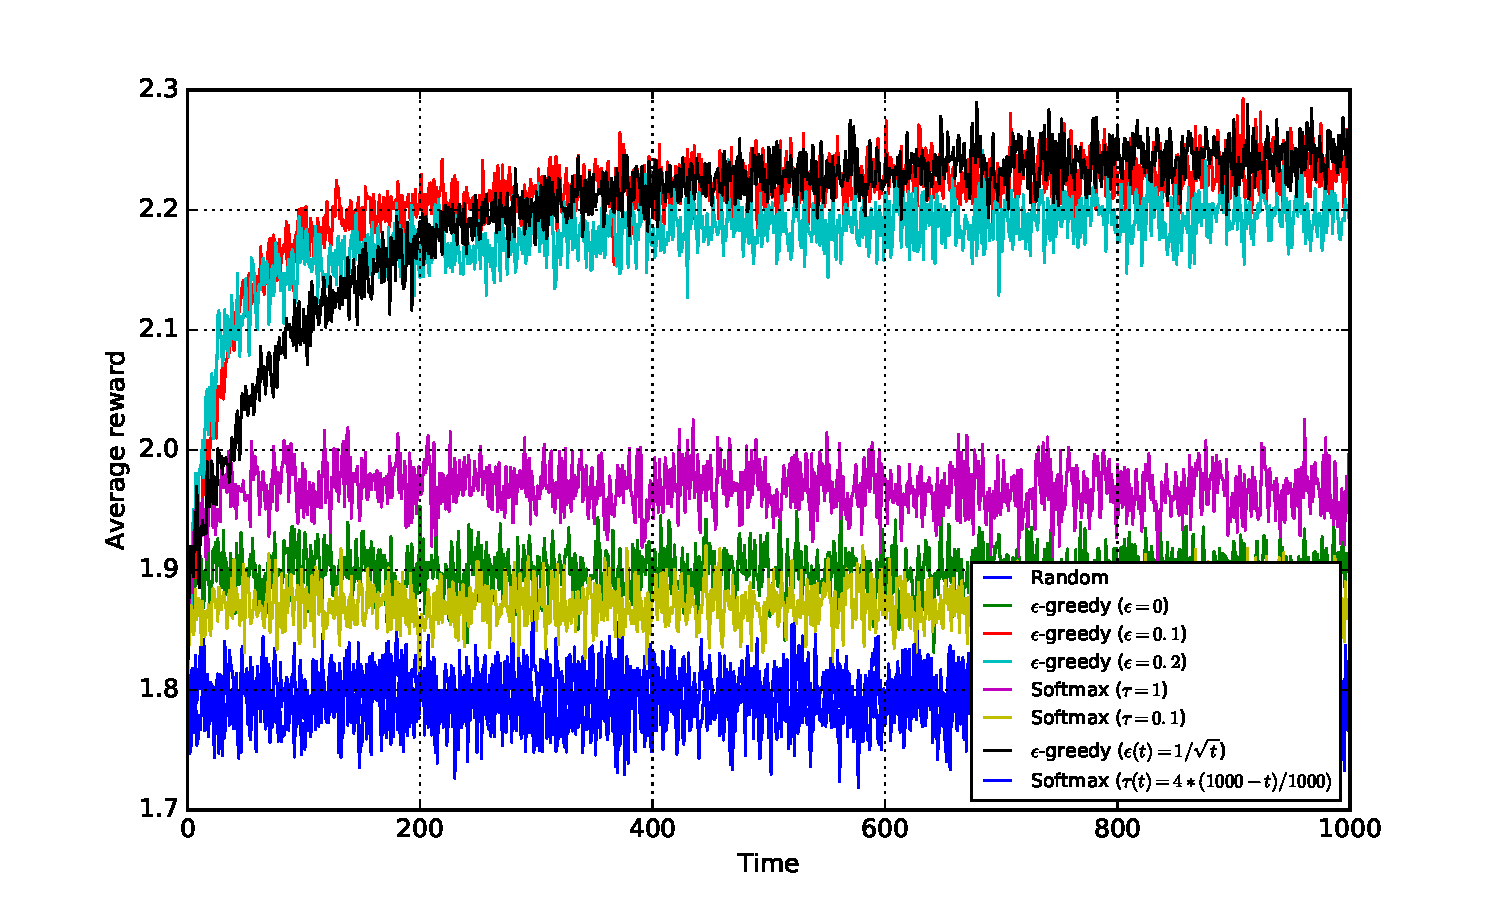
\includegraphics[width=0.7\textwidth]{./fig/ex1-3.pdf}
	\caption{Evolution of the average reward over 10000 runs during training}
	\label{ex13perf}
\end{figure}
\begin{figure}[H]
	\centering
	\subfloat[][Arm 1]{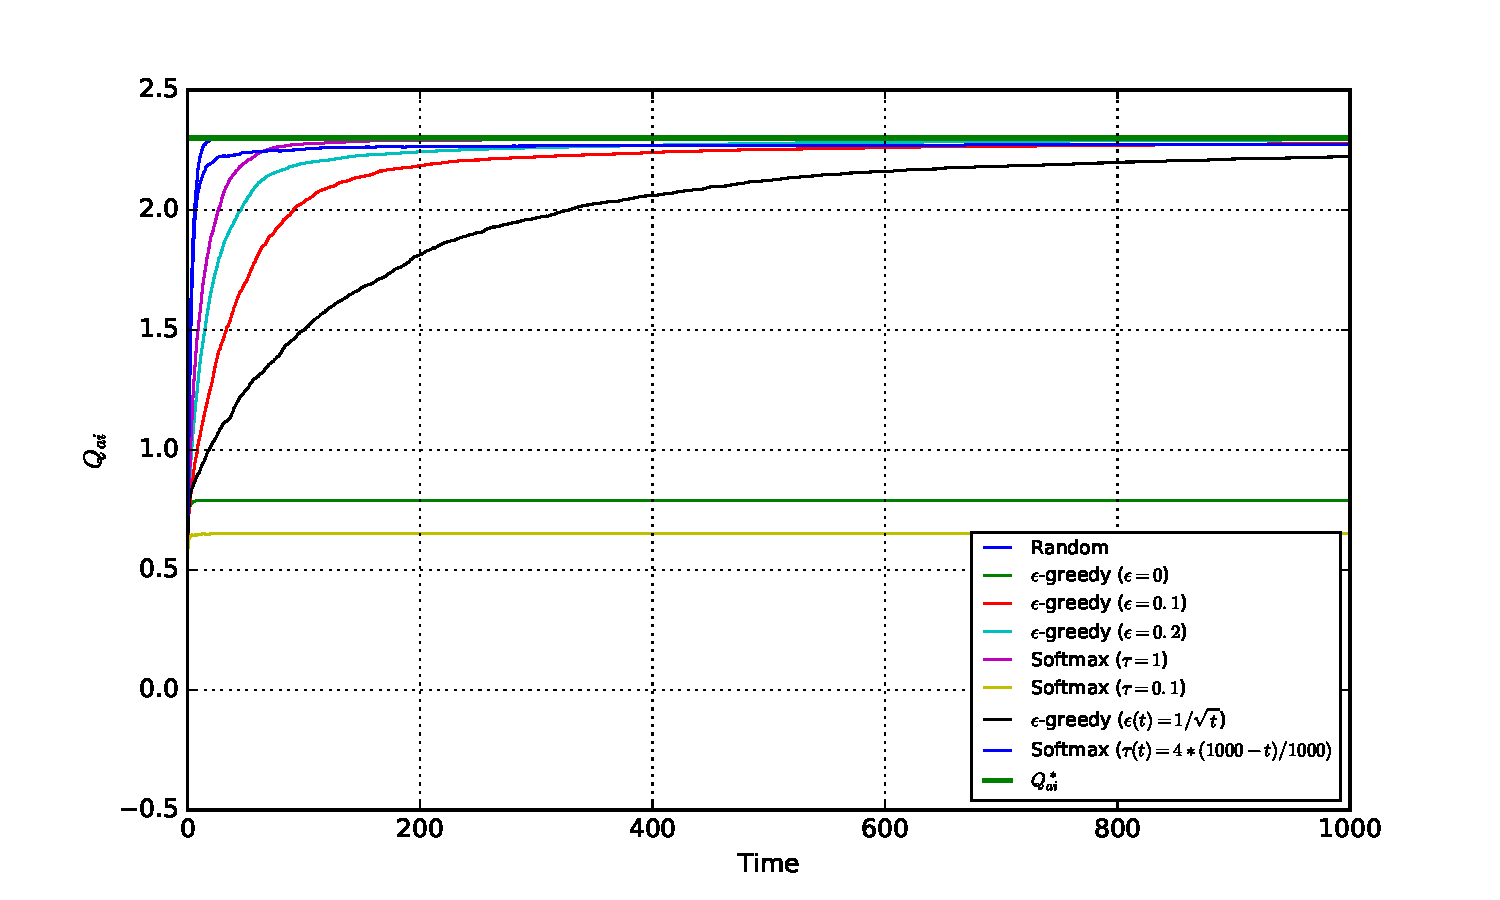
\includegraphics[width=.49\textwidth]{./fig/ex1-3-q0.pdf}}
	\subfloat[][Arm 2]{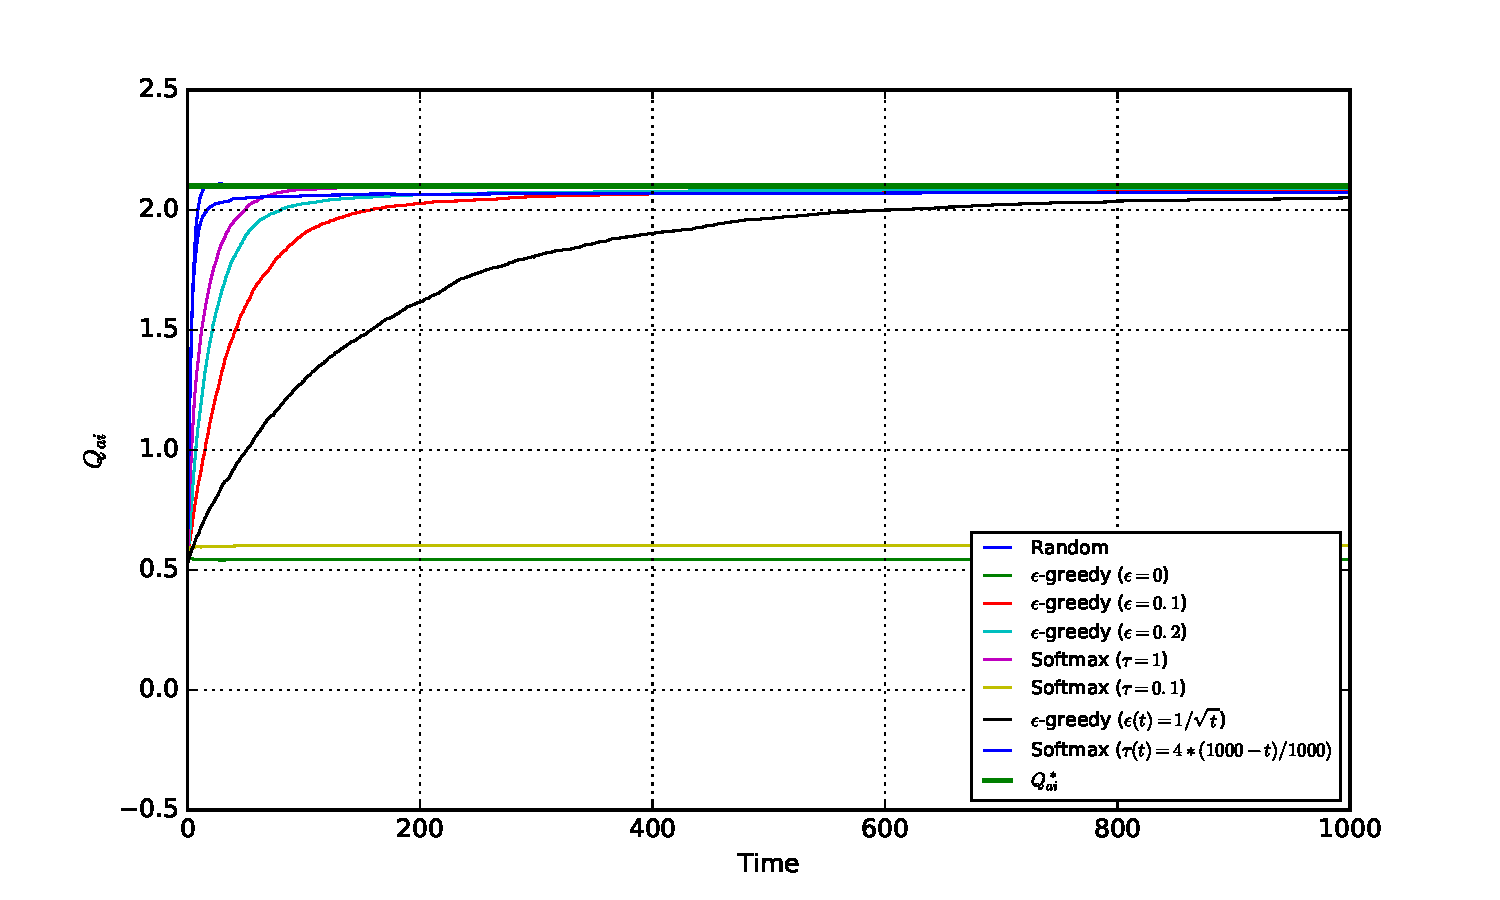
\includegraphics[width=.49\textwidth]{./fig/ex1-3-q1.pdf}}
	\\
	\subfloat[][Arm 3]{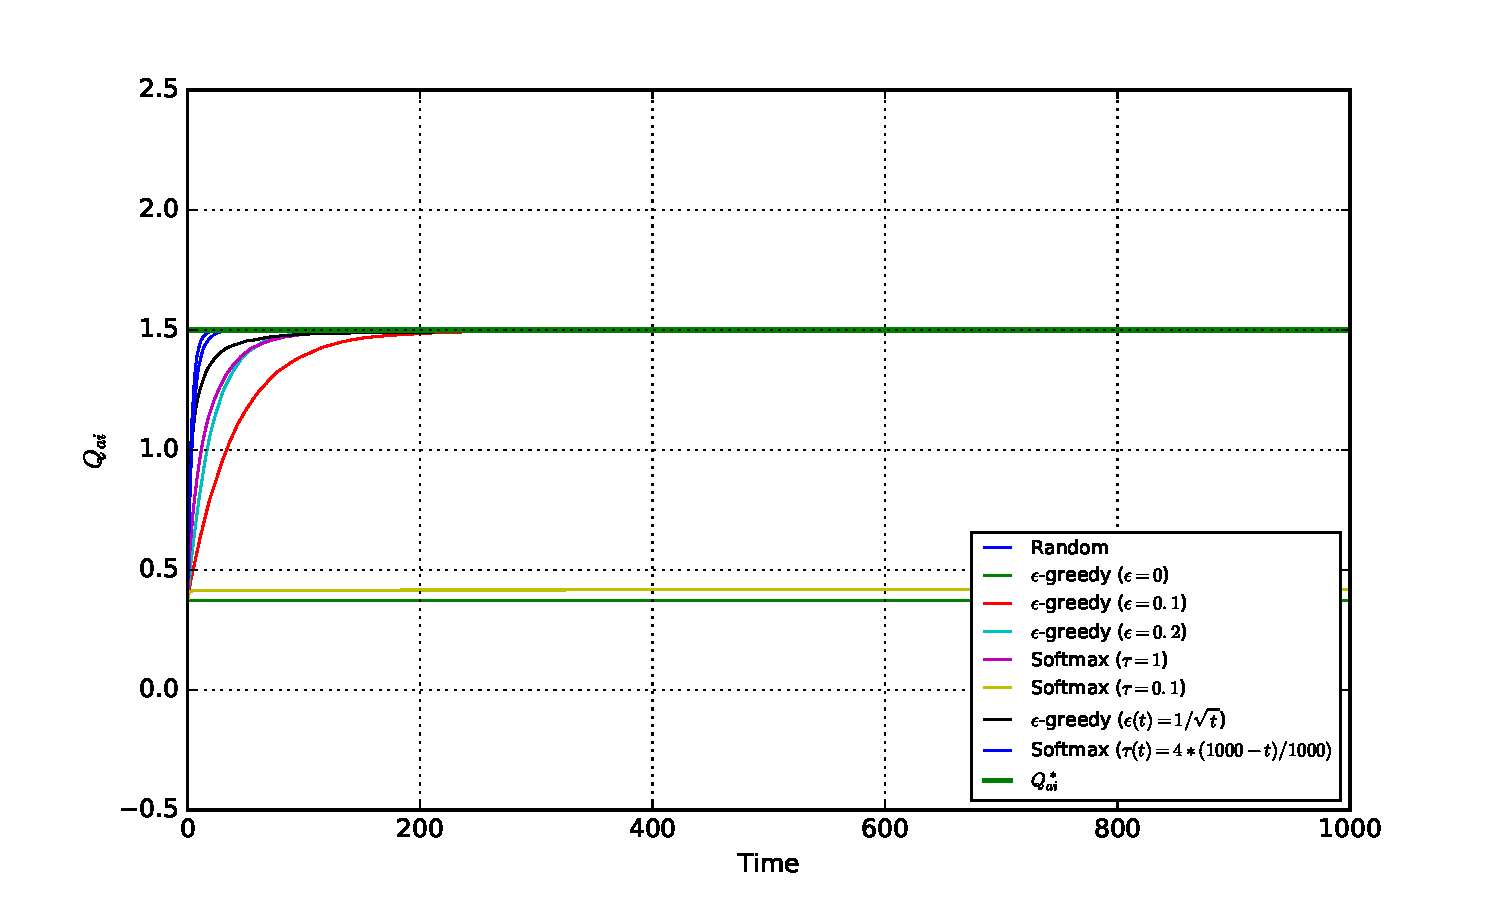
\includegraphics[width=.49\textwidth]{./fig/ex1-3-q2.pdf}}
	\subfloat[][Arm 4]{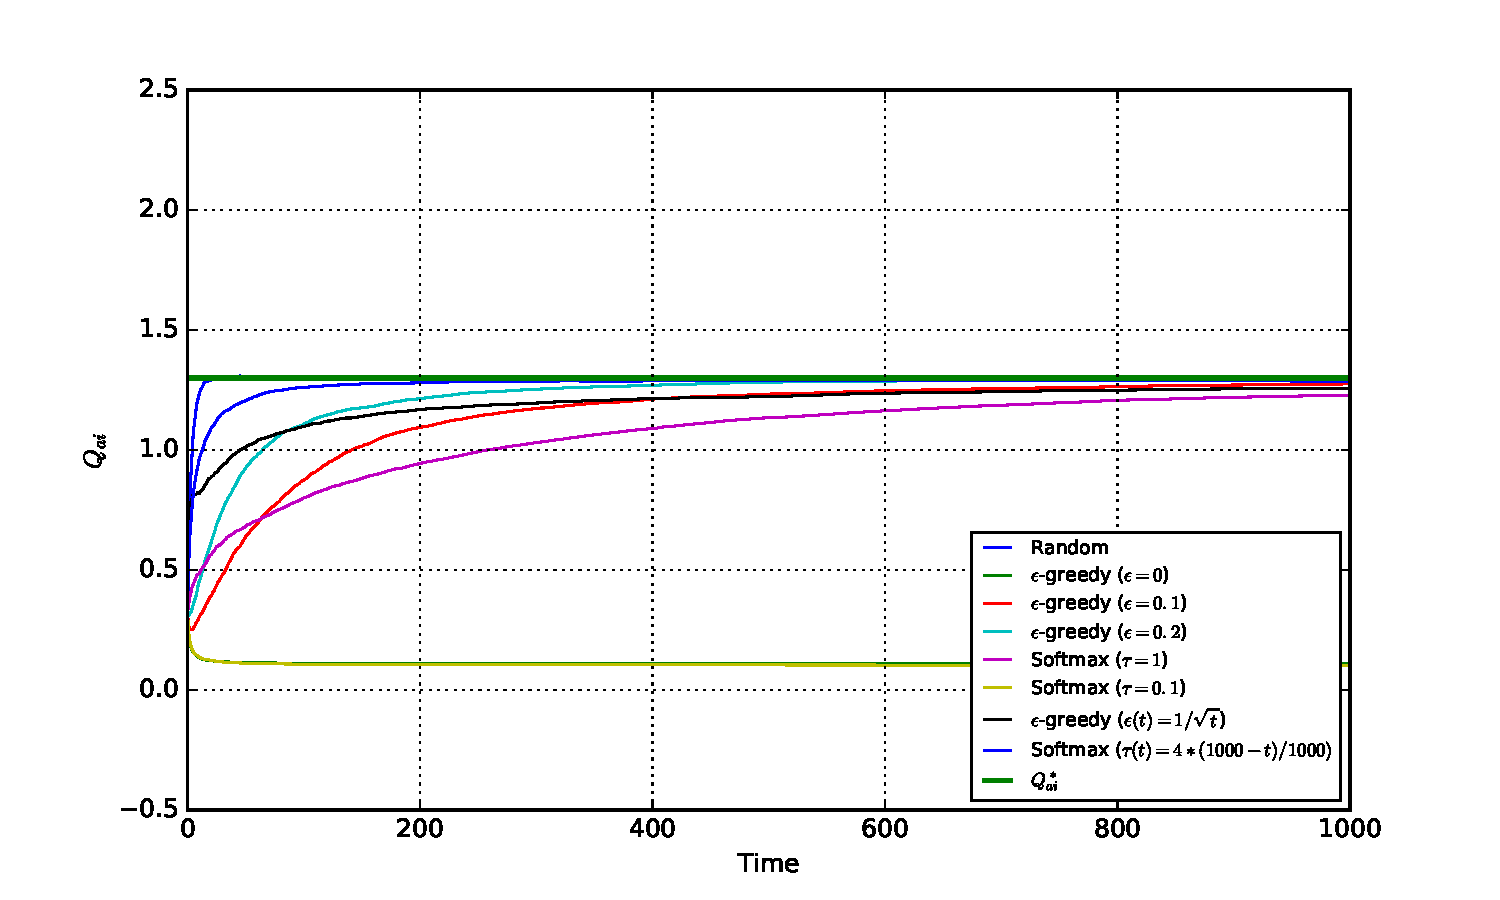
\includegraphics[width=.49\textwidth]{./fig/ex1-3-q3.pdf}}
	\caption{Evolution of $Q_{ai}$ for each arm}
	\label{ex13q}
\end{figure}

Once again, the graphs in figure \ref{ex13a} do not show the full picture.
The graph for Softmax with a varying $\tau$ doesn't show that once it has 
learned a good estimation of all $Q^*_{ai}$ and the temperature is decreased,
it will always choose the optimal arm.\\

Looking at figure \ref{ex13q}, it is clear that Softmax with a varying $\tau$
is the quickest (except for the random policy) to learn about the Q values.
We could decrease the temperature much earlier to reach optimal rewards.

\begin{figure}[H]
	\centering
	\subfloat[][Random]{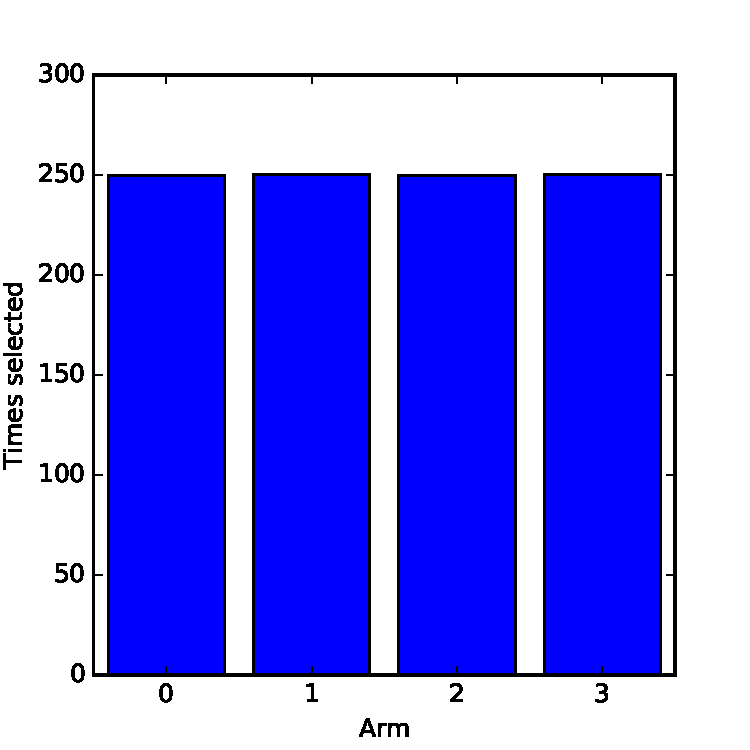
\includegraphics[width=.16\textwidth]{./fig/ex1-3-a0.pdf}}
	\subfloat[][$\epsilon$-greedy 0]{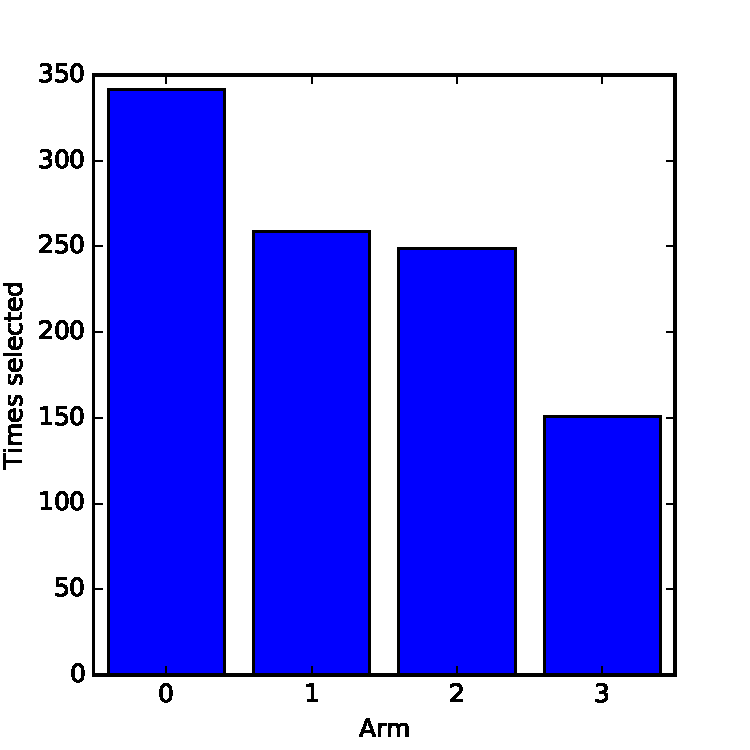
\includegraphics[width=.16\textwidth]{./fig/ex1-3-a1.pdf}}
	\subfloat[][$\epsilon$-greedy 0.1]{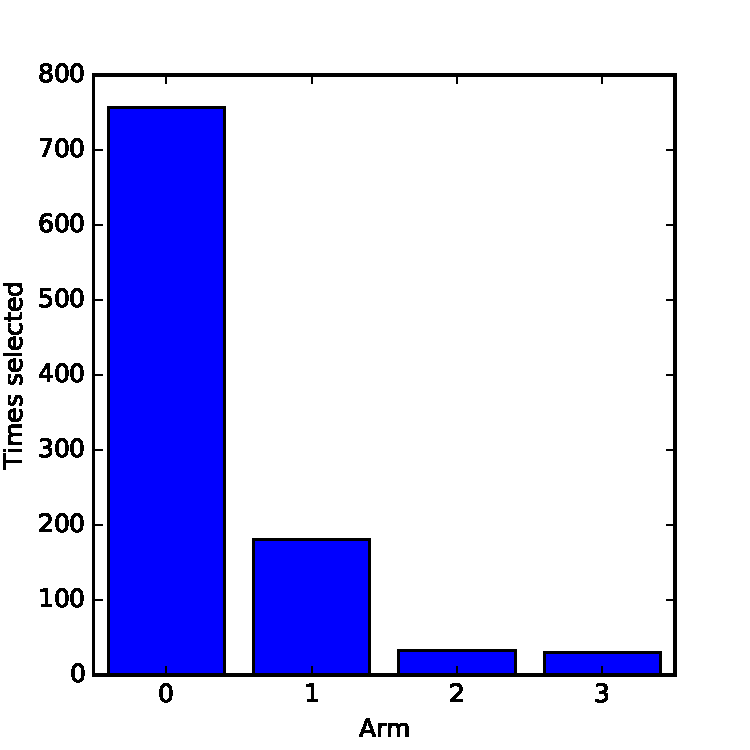
\includegraphics[width=.16\textwidth]{./fig/ex1-3-a2.pdf}}
	\subfloat[][$\epsilon$-greedy 0.2]{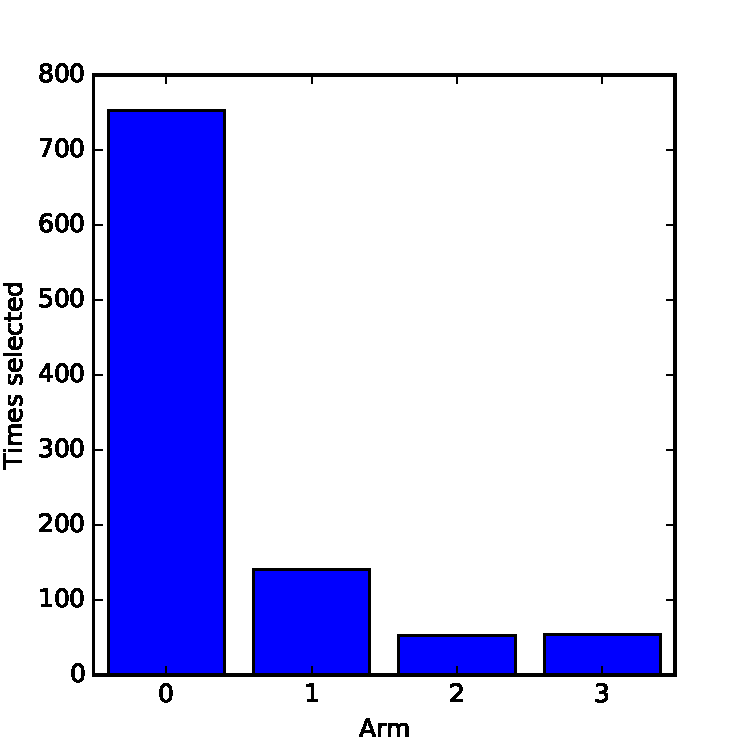
\includegraphics[width=.16\textwidth]{./fig/ex1-3-a3.pdf}}
	\\
	\subfloat[][Softmax 1]{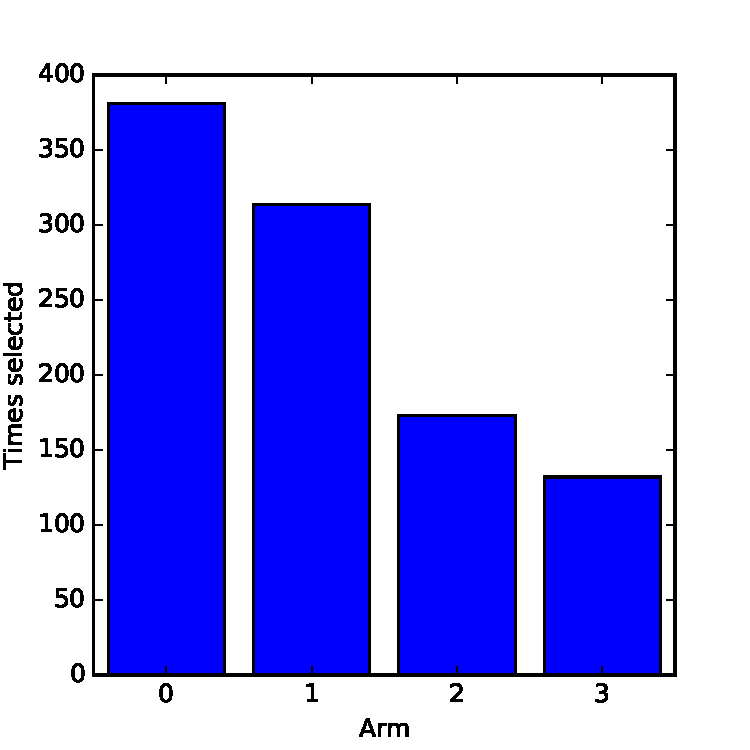
\includegraphics[width=.16\textwidth]{./fig/ex1-3-a4.pdf}}
	\subfloat[][Softmax 0.1]{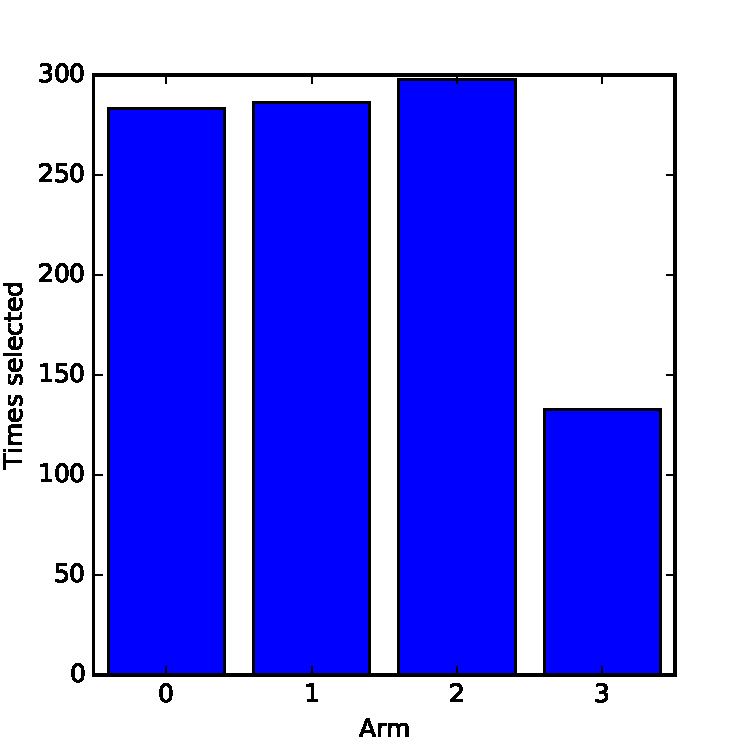
\includegraphics[width=.16\textwidth]{./fig/ex1-3-a5.pdf}}
	\subfloat[][$\epsilon(t)$]{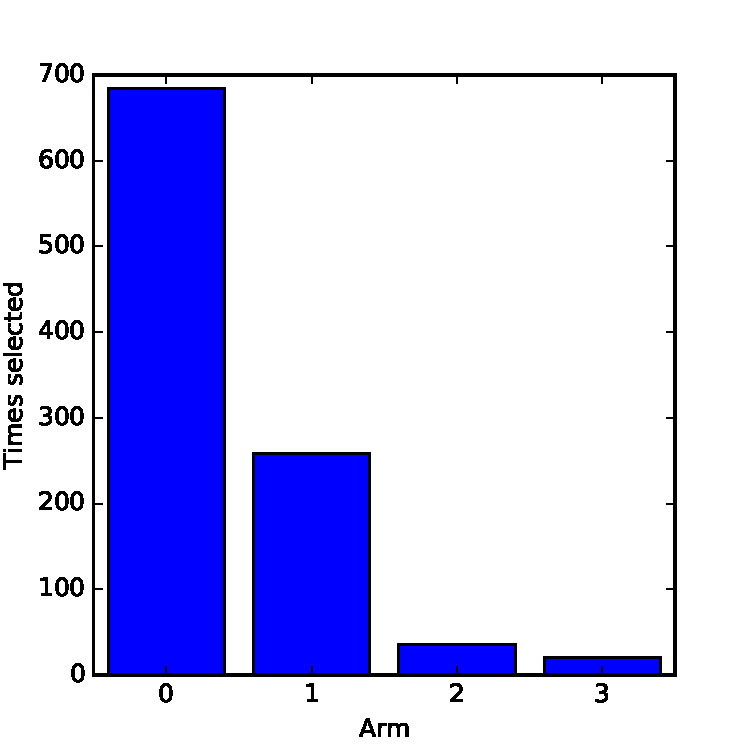
\includegraphics[width=.16\textwidth]{./fig/ex1-3-a6.pdf}}
	\subfloat[][$\tau(t)$]{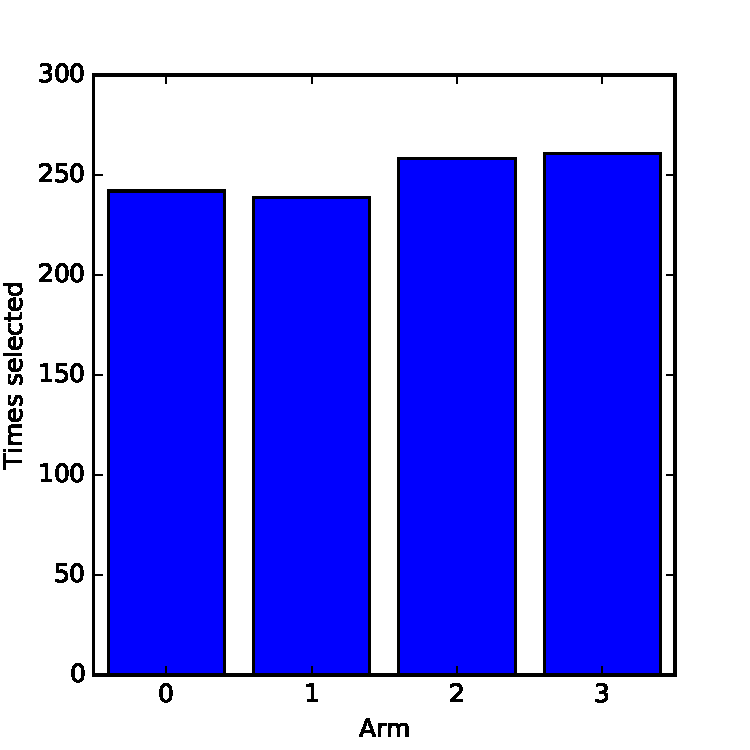
\includegraphics[width=.16\textwidth]{./fig/ex1-3-a7.pdf}}
	\caption{Actions taken by each algorithm}
	\label{ex13a}
\end{figure}

\section{Stochastic Reward Game}
Two agents play a game where both try to maximise the reward they get from
joint actions. The game is the stochastic climbing game :

\begin{table}[H]
\centering
\begin{tabular}{c|c|c|c}
	& $a_1$ & $a_2$ & $a_3$ \\ \hline
	$b_1$ & $\mathcal{N}(11, \sigma_0^2)$ & $\mathcal{N}(-30, \sigma^2)$
		& $\mathcal{N}(0, \sigma^2)$ \\ \hline 
	$b_2$ & $\mathcal{N}(-30, \sigma^2)$ & $\mathcal{N}(7, \sigma_1^2)$
		& $\mathcal{N}(6, \sigma^2)$ \\ \hline 
	$b_3$ & $\mathcal{N}(0, \sigma^2)$ & $\mathcal{N}(0, \sigma^2)$
		& $\mathcal{N}(5, \sigma^2)$ 
\end{tabular}
\caption{The stochastic climbing game}
\label{banditparams}
\end{table}

We use the standard method described in \cite{claus} which consists of doing
Boltzmann exploration using expected values considering the probabilities that
the other player will play each action.\\

The heuristic chosen is optimistic Boltzmann. All graphs are smoothed with
an exponential average :
$$ \widehat{x}_{t+1} = (1-\alpha)\widehat{x}_t + \alpha * x $$
with $\alpha = 0.02$. \\

As we can see on figure \ref{ex31perf}, the first type converges
to a reward of 7. This is the expected equilibrium as shown in figures 3, 4 and
5 in \cite{claus}. However, we also see that the heuristic manages to overcome
the 'fear' of getting a large negative reward by being optimistic and 
converges to 11.\\

When the highest reward is made more uncertain, the optimistic reward seems
to converge to about 7 as well. However, if we make the reward for 
<$a_2$, $b_2$> more uncertain, both algorithms will end up choosing this action
and will receive a reward with very high variance (as can be seen from the
much less stable plot)\\


\begin{figure}[H]
	\centering
	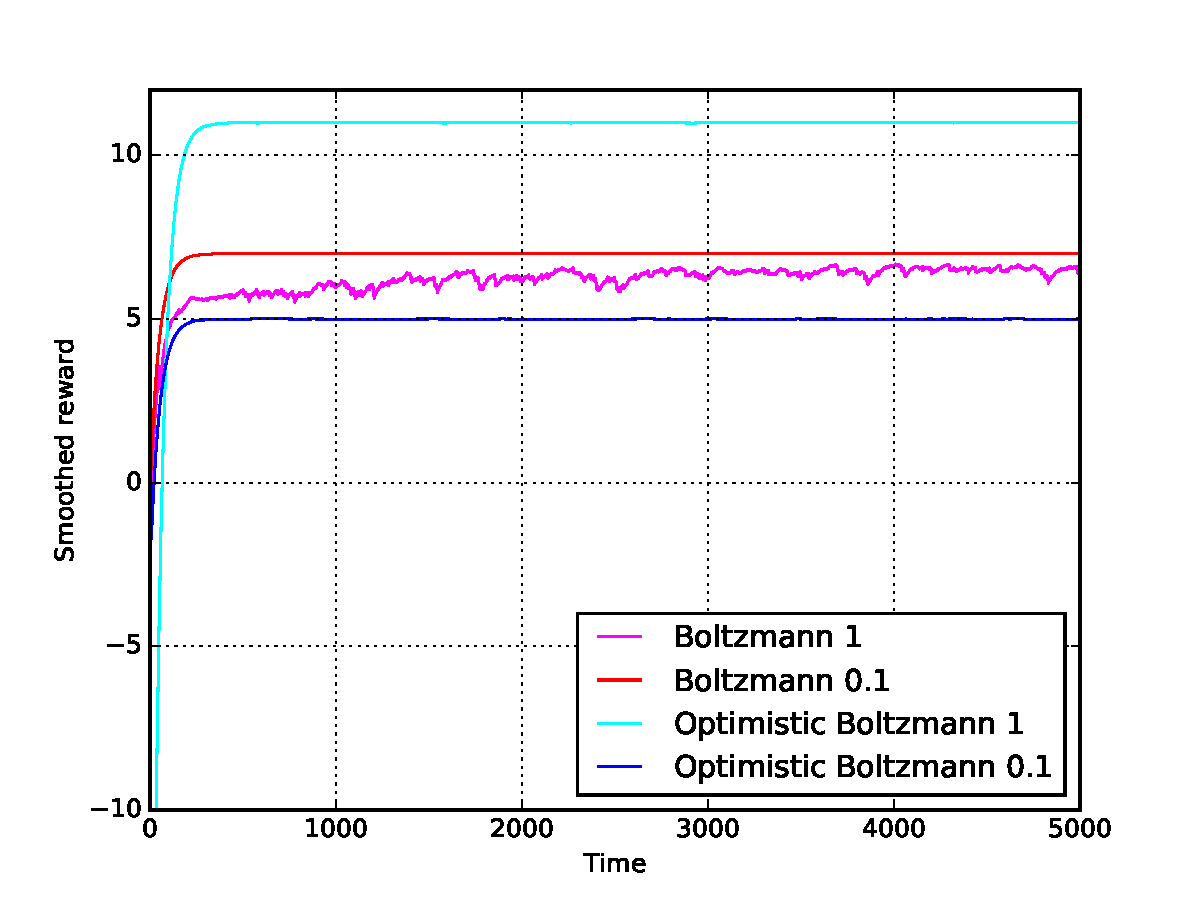
\includegraphics[width=0.7\textwidth]{./fig/ex2-0.pdf}
	\caption{Evolution of the average reward during training with 
		$\sigma_0 = \sigma_1 = \sigma = 0.2$}
	\label{ex31perf}
\end{figure}
\begin{figure}[H]
	\centering
	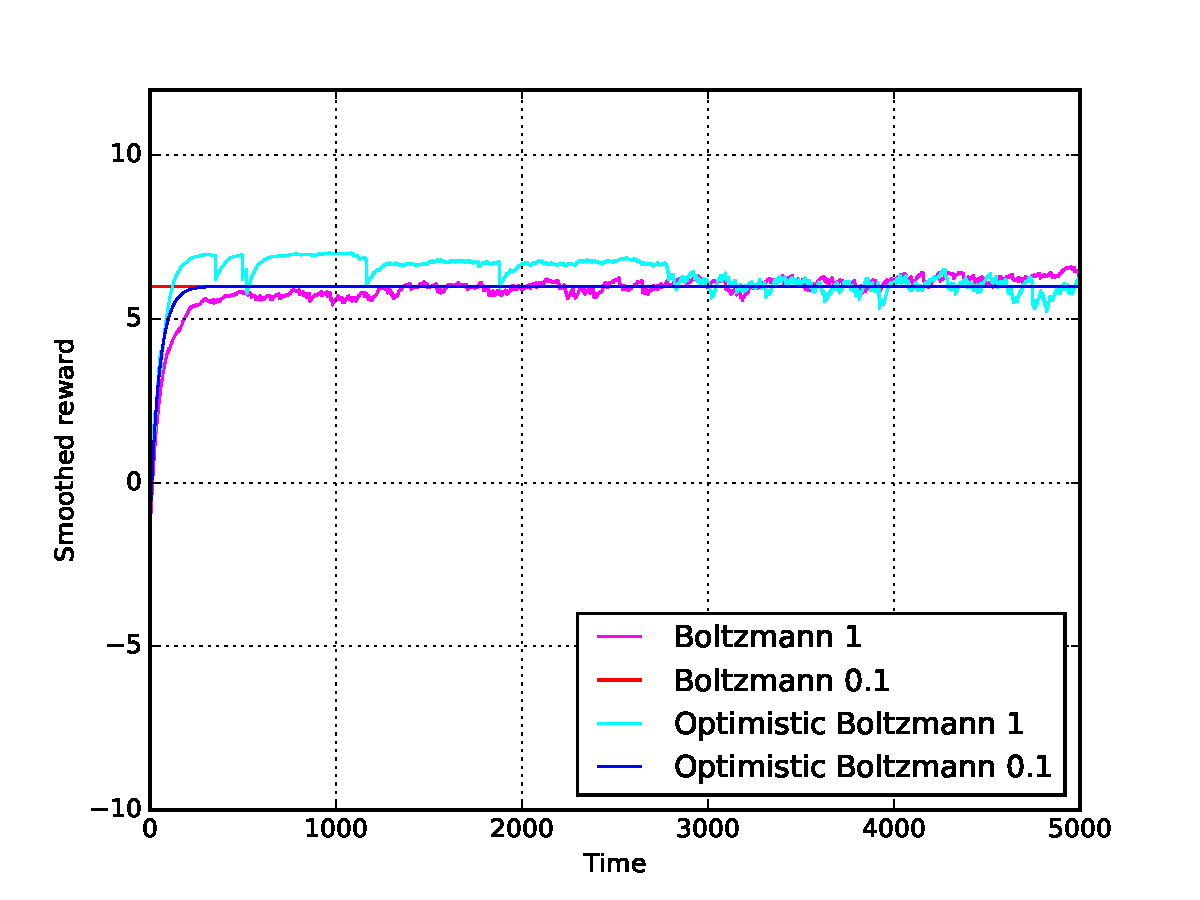
\includegraphics[width=0.7\textwidth]{./fig/ex2-1.pdf}
	\caption{Evolution of the average reward during training with
		$\sigma_0 = 4$ and $\sigma_1 = \sigma = 0.1$}
	\label{ex32perf}
\end{figure}
\begin{figure}[H]
	\centering
	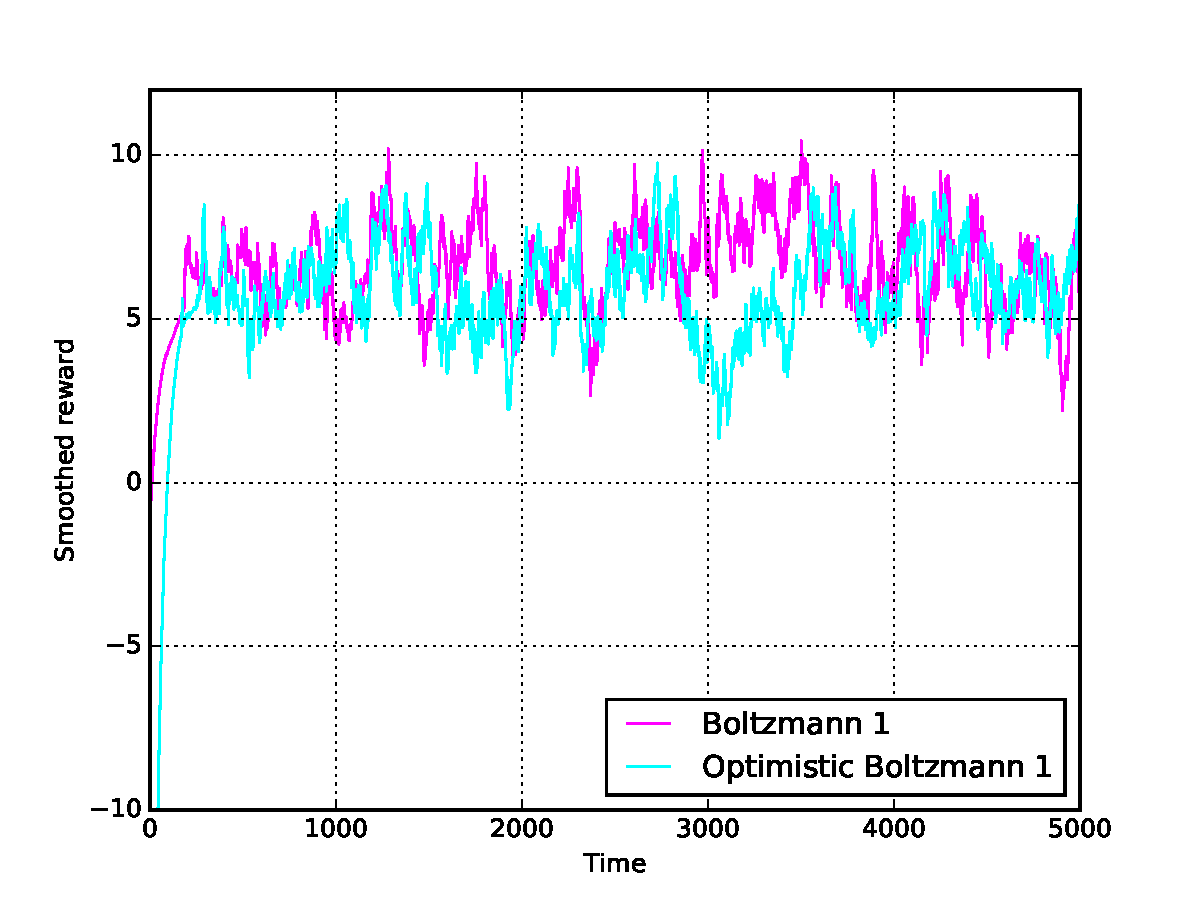
\includegraphics[width=0.7\textwidth]{./fig/ex2-2.pdf}
	\caption{Evolution of the average reward during training with
		$\sigma_1 = 4$ and  $\sigma_0 = \sigma = 0.1$}
	\label{ex33perf}
\end{figure}

\begin{thebibliography}{1}
	\bibitem{claus} C. Claus and C. Boutilier. The dynamics of 
		reinforcement learning in cooperative multiagent systems. 
		\textit{AAAI/IAAI}, (s 746):752, 1998.
\end{thebibliography}

\appendix
\section{N-Armed Bandit code}
\inputminted{python}{partone.py}

\section{Stochastic Reward Game code}
\inputminted{python}{parttwo.py}
\end{document}
